\documentclass[journal]{style/vgtc} 			          % final (journal style)
%\documentclass[review,journal]{style/vgtc}         % review (journal style)
%\documentclass[widereview]{style/vgtc}             % wide-spaced review
%\documentclass[preprint,journal]{style/vgtc}       % preprint (journal style)
%\documentclass[electronic,journal]{style/vgtc}     % electronic version, journal
%% Uncomment one of the lines above depending on where your paper is
%% in the conference process. ``review'' and ``widereview'' are for review
%% submission, ``preprint'' is for pre-publication, and the final version
%% doesn't use a specific qualifier. Further, ``electronic'' includes
%% hyperreferences for more convenient online viewing.
%% Please use one of the ``review'' options in combination with the
%% assigned online id (see below) ONLY if your paper uses a double blind
%% review process. Some conferences, like IEEE Vis and InfoVis, have NOT
%% in the past.

%% Please note that the use of figures other than the optional teaser is not permitted on the first page
%% of the journal version.  Figures should begin on the second page and be
%% in CMYK or Grey scale format, otherwise, colour shifting may occur
%% during the printing process.  Papers submitted with figures other than the optional teaser on the
%% first page will be refused.

%% These three lines bring in essential packages: ``mathptmx'' for Type 1
%% typefaces, ``graphicx'' for inclusion of EPS figures. and ``times''
%% for proper handling of the times font family.

\usepackage{mathptmx}
\usepackage{graphicx}
\usepackage{times}

% -- My Own Packages and Commands
\usepackage[normalem]{ulem}
\usepackage{xcolor}
\newcommand{\rem}[1]{\textcolor{red}{\sout{#1}}}
\newcommand{\add}[1]{\textcolor{blue}{#1}}
\newcommand{\com}[1]{\textcolor{red}{#1}}
\newcommand{\design}[1]{\textcolor{orange}{#1}}
\newcommand{\magenta}[1]{\textcolor{magenta}{#1}}
% white, black, red, green, blue, cyan, magenta, yellow.

%% We encourage the use of mathptmx for consistent usage of times font
%% throughout the proceedings. However, if you encounter conflicts
%% with other math-related packages, you may want to disable it.

%% This turns references into clickable hyperlinks.
\usepackage[bookmarks,backref=true,linkcolor=black]{hyperref} %,colorlinks
\hypersetup{
  pdfauthor = {},
  pdftitle = {},
  pdfsubject = {},
  pdfkeywords = {},
  colorlinks=true,
  linkcolor= black,
  citecolor= black,
  pageanchor=true,
  urlcolor = black,
  plainpages = false,
  linktocpage
}

%% If you are submitting a paper to a conference for review with a double
%% blind reviewing process, please replace the value ``0'' below with your
%% OnlineID. Otherwise, you may safely leave it at ``0''.
\onlineid{175}

%% declare the category of your paper, only shown in review mode
\vgtccategory{Research}

%% allow for this line if you want the electronic option to work properly
\vgtcinsertpkg

%% In preprint mode you may define your own headline.
%\preprinttext{To appear in an IEEE VGTC sponsored conference.}

%% Paper title.

\title{3D Regression Heat Map Analysis of Population Study Data}

%% This is how authors are specified in the journal style

%% indicate IEEE Member or Student Member in form indicated below
\author{Paul Klemm, Kai Lawonn, Sylvia Gla{\ss}er, Uli Niemann, Katrin Hegenscheid, Henry V{\"o}lzke, Bernhard Preim}
\authorfooter{
%% insert punctuation at end of each item
\item
 Paul Klemm, Sylvia Gla{\ss}er, Uli Niemann, Bernhard Preim are with Otto-von-Guericke University Magdeburg, Germany. E-mail: \{klemm,lawonn,glasser,uli.niemann,preim\}@ovgu.de
\item
 Katrin Hegenscheid, Henry V{\"o}lzke are with Ernst-Moritz-Arndt University Greifswald, Germany. E-mail: \{katrin.hegenscheid,voelzke\}@uni-greifswald.de
\item
 Kai Lawonn is with Otto-von-Guericke University Magdeburg, Germany and Delft University of Technology, Delft, Netherlands. E-mail: lawonn@ovgu.de
}

%other entries to be set up for journal
\shortauthortitle{Klemm \MakeLowercase{\textit{et al.}}: 3D Regression Heat Map Analysis of Population Study Data}
%\shortauthortitle{Firstauthor \MakeLowercase{\textit{et al.}}: Paper Title}

%% Abstract section.
\abstract{%
%\com{Problem}.
Epidemiological studies comprise heterogeneous data about a subject group to define disease-specific risk factors.
%%
These data contain information (\emph{features}) about a subject's lifestyle, medical status as well as medical image data.
%%
Statistical regression analysis is used to evaluate these features and to identify feature combinations indicating a disease (the \emph{target feature}).
%%
%Although there is a strong demand for overview visualizations of a whole data set w.r.t. a target feature, no suitable tool is available for epidemiological researchers.

%\com{New Solution}.
%%
We propose an analysis approach of epidemiological data sets by incorporating all features in an exhaustive regression-based analysis.
%%
This approach combines all \emph{independent features} w.r.t. a \emph{target feature}.
%%
It provides a visualization that reveals insights into the data by highlighting relationships.
%%
The \emph{3D Regression Heat Map}, a novel 3D visual encoding, acts as an overview of the whole data set.
%%
It shows all combinations of two to three independent features with a specific target disease.
%%
%A 3D visualization of all combinations of two to three independent features towards a target acts as an overview of the whole data set, the \emph{3D Regression Heat Map}.
%%
Slicing through the \emph{3D Regression Heat Map} allows for the detailed analysis of the underlying relationships.
%%
Expert knowledge about disease-specific hypotheses can be included into the analysis by adjusting the regression model formulas.
%%
Furthermore, the influences of features can be assessed using a difference view comparing different calculation results.
%%
%\com{Validation \& Results}.
%%
We applied our \emph{3D Regression Heat Map} method to a hepatic steatosis data set to reproduce results from a data mining-driven analysis.
%%
A qualitative analysis was conducted on a breast density data set.
%%
We were able to derive new hypotheses about relations between breast density density and breast lesions with breast cancer.
%%
%\com{Implications}.
%%
With the \emph{3D Regression Heat Map}, we present a visual overview of epidemiological data that allows for the first time an interactive regression-based analysis of large feature sets with respect to a disease.
} % end of abstract

%% Keywords that describe your work. Will show as 'Index Terms' in journal
%% please capitalize first letter and insert punctuation after last keyword
\keywords{Interactive Visual Analysis, Regression Analysis, Heat Map, Epidemiology, Breast Cancer, Hepatic Steatosis}

%% ACM Computing Classification System (CCS).
%% See <http://www.acm.org/class/1998/> for details.
%% The ``\CCScat'' command takes four arguments.

\CCScatlist{ % not used in journal version
 \CCScat{K.6.1}{Management of Computing and Information Systems}%
{Project and People Management}{Life Cycle};
 \CCScat{K.7.m}{The Computing Profession}{Miscellaneous}{Ethics}
}

%% Uncomment below to include a teaser figure.
  % \teaser{
  % \centering
  % \includegraphics[width=16cm]{CypressView}
  % \caption{In the Clouds: Vancouver from Cypress Mountain.}
  % }

%% Uncomment below to disable the manuscript note
%\renewcommand{\manuscriptnotetxt}{}

%% Copyright space is enabled by default as required by guidelines.
%% It is disabled by the 'review' option or via the following command:
% \nocopyrightspace

%%%%%%%%%%%%%%%%%%%%%%%%%%%%%%%%%%%%%%%%%%%%%%%%%%%%%%%%%%%%%%%%
%%%%%%%%%%%%%%%%%%%%%% START OF THE PAPER %%%%%%%%%%%%%%%%%%%%%%
%%%%%%%%%%%%%%%%%%%%%%%%%%%%%%%%%%%%%%%%%%%%%%%%%%%%%%%%%%%%%%%%

\begin{document}

%% The ``\maketitle'' command must be the first command after the
%% ``begin{document}'' command. It prepares and prints the title block.

%% the only exception to this rule is the \firstsection command
\firstsection{Introduction}

\maketitle
%%
Epidemiology aims to characterize health and disease conditions in defined populations (\emph{cohorts}).
%%
Insights about risk factors allow to characterize disease-specific high-risk groups \cite{Fletcher2012}.
%%
Furthermore, the insights can be used to derive recommendations regarding a healthy lifestyle or to provide information about widespread diseases.
%%
During the standard workflow, physicians transform observations into hypotheses.
%%
The hypotheses are depicted using epidemiological features and are then statistically analyzed.

%An important epidemiological tool for deriving such features is the evaluation of a \emph{cohort study}, such as the Study of Health in Pomerania (SHIP) \cite{Volzke2011}.
An important epidemiological tool for deriving such features are \emph{cohort studies}, such as the Study of Health in Pomerania (SHIP) \cite{Volzke2011}.
%%
To reduce any selection bias, subjects are randomly invited without a focus on a specific disease.
%%
Hence, a wide range of features is acquired.
%
Social and lifestyle factors, prior or current diseases and medications as well as medical parameters, such as blood pressure, are gathered.
%%
%Medical image data from non-radiating modalities, e.g., magnetic resonance imaging (MRI), is also acquired in modern studies.
%%
%These data may be quantified based on user-defined landmarks, which describe attributes like the shape, volume or diameter of a structure.
%%

Testing features for associations with diseases using regression models is one of the most important epidemiological tools.
%%
Using regression analysis to assess the statistical resilience of a hypothesis rarely involves \emph{more than three features} due to the higher dimensional problem and the required subject count.
%%
Due to the amount of data and only limited overview visualizations, possible correlations may be missed.
%%
Explorative analyses and overview visualizations of the data set as presented in prior work \cite{Klemm2014VIS} are not tailored to a specific target feature.
%%
They mostly highlight correlations between features, which are known to the domain expert (e.g., correlation between body size and spine shape).
%%
We incorporate the regression analysis, which is familiar to the domain experts, into overview visualizations to support a hypothesis-free analysis or an analysis w.r.t. a specific disease or hypothesis.
%%
For this purpose we provide template regression formulas, which are applied to all potential feature combinations.
%%
Since the notation is familiar to epidemiologists, they can rapidly include their domain knowledge into the analysis process.
%%
Difference views between regression formulas allow to assess the influences of individual features on the process.
%%
Our contributions are:

\design{
\begin{itemize}
	%%
  \item An overview visualization design based on feedback of epidemiological domain experts to support hypothesis-generation w.r.t. a target feature using regression models.
	%%
  \item Applying domain knowledge in the analysis using freely adjustable regression formulas.
	%%
  \item Selecting suitable metrics for representing and comparing regression models, as well as incorporating additional metrics for details-on-demand to assess the model quality.
	%%
  \item An openly available web-based system, which incorporates open formats to be applicable for data of other application domains.
	%%
\end{itemize}
}
% \begin{itemize}
% 	%%
% 	\item An overview visualization technique representing feature interactions using target features.
% 	%%
% 	\item Visualization techniques, which incorporate overview visualizations of all regression analyses at once as well as details-on-demand techniques for in-depth investigations of feature relationships.
% 	%%
% 	\item Freely adjustable regression formulas to provide a simple, yet powerful way to adjust the regression analysis to specific hypotheses about the data.
% 	%%
% 	\item The analysis of confounding features by providing comparison views between different formula results.
% 	%%
% 	\item The expansion and adaption of our method to any data with our open web-based system.
% 	%%
% \end{itemize}
%%
% \noindent The term `Regression Cube' has been used for the detailed analysis of one or a small number of regression models \cite{Ahmadi, Chan}.
% %%
% They extend 2D scatter plots to display detailed information about a regression model.
% %%
% In behalf of that, we declare our visualization technique for comparing and analyzing a large number of different regression models with different input features as \emph{Regression Cube}.
% %%
\section{Epidemiological Background} \label{sec:Background}
%%
This section covers the epidemiological workflow, epidemiological data in general and the SHIP in particular.
%%
\subsection{Epidemiological Workflow} \label{sec:EpidemiologicalWorkflow}
%%
Epidemiological research is performed by experts from different academic disciplines, such as epidemiologists, physicians, statisticians, and medical computer scientists focusing on biometrics and image segmentation.
%%
Their goal is to derive disease-specific risk factors by assessing epidemiological features with statistical methods.
%%
As described by Thew et al.~\cite{Thew2009} the epidemiological workflow is divided into these different steps:
\begin{enumerate}
	\item Clinicians/Epidemiologists derive hypotheses via clinical observations, experimental studies or literature research.
	%\item Clinicians make observations in the daily practice, which are translated into hypotheses.
	\item Epidemiologists compile a list of features depicting the hypothesis and include confounding features.
	\item Statisticians assess the association of the derived features w.r.t the investigated disease.
\end{enumerate}
%%
Relative risks can be determined if a statistical resilient association of features with a condition is extracted.
%%
Derived absolute risks indicate the per-subject chance of developing the disease.
%%
Reproducibility of results is an epidemiological key requirement and guides all analyses steps.
%%
Statistical programs, such as \texttt{SPSS}, are used to analyze the data regarding the classical sequential epidemiological workflow.
%%
Hence, images are mostly used for the communication of results, rather than for providing insight into the data.
%%

We described an Interactive Visual Analysis approach for image-centric cohort study data, which connects to the feature listing step \cite{Klemm2014VIS}.
%%
The methods aim to derive hypotheses through analysis of the data and observations about previously unknown feature correlations.
%%
\emph{Hypothesis generation} benefits from overview visualizations of feature correlations, which are not supported by standard statistical processors.
%%
In this work, we focus on a similar approach to derive insight and even new hypotheses through the data rather than only using it for a confirmatory analysis.
%%
\subsection{Epidemiological Data} \label{sec:EpidemiologicalData}
%%
There are many epidemiological instruments available to acquire data. %, which are suitable for different analysis types.
%%
We focus on population studies, which impose the largest data sets and yield a highly heterogenous and incomplete information space.
%%
Subject data are collected either regarding specific diseases or with the widest range possible.
%%
The latter allows the data set to be assessed w.r.t. different diseases.
%%
The feature space comprises information about lifestyle, somatometric features, medical parameters, genetic data as well as medical images.
%%
These features are gathered through questionnaires, medical examinations and laboratory analyses.
%%
Many features are sparse, such as follow-up questions about a medication or treatment of a certain disease.
%%
Other features are exclusive for a sub-group, such as women-specific questions, e.g., number of born children or period status.
%%
Medical status features or lifestyle factors are primarily of \emph{dichotomous} (binary) type.
%%
Continuous data are often discretized (e.g. 10 year steps for age) to equalize the feature types and to simplify the method selection.
%%
However, this reduces the information space and introduces a information bias, as assumptions are modeled through the discretization.
%%

Medical image data are also analyzed in modern population studies.
%%
We incorporate image-derived features, but do not focus on analyzing image data.
%%
More discussions of population study data types and characteristics can be found in the works of Preim et al.~\cite{Preim2014} and Toennies et al.~\cite{Toennies2015}.
%%

Features influencing the exposure as well as the outcome of an analysis are called \emph{confounders} and have to be specially treated.
%%
The analysis model has to be adjusted by normalizing all included features w.r.t. the confounder.
%%
\emph{Age} is included as confounder in almost any epidemiological analysis, since most diseases are more likely for older subjects.
%% TODO Shorten next sentence if needed
It also influences the general body condition and thereby almost all features acquired through population studies.
%%
Another important confounder is \emph{gender}.
%%
Confounders have to be selected by epidemiologists specific to the investigated condition.
%%
\paragraph{The Study of Health in Pomerania (SHIP).}
The \texttt{SHIP}, located in Northern Germany, aims to characterize health and disease in the widest range possible \cite{Volzke2011}.
%%
%It does not focus on a specific disease, making the data set open for many diseases.
%%
Unique for the \texttt{SHIP} is the acquisition of medical image data.
%%
A second cohort, \texttt{SHIP-TREND} was started in 2012.
%%
Data for both cohorts are examined in a 5-year time span.
%%
New parameters are added in each iteration, extending the range of investigated diseases.
%%
%For the latest two acquisitions (\texttt{SHIP-2} and \texttt{SHIP-TREND-0}), MRI scans are included into the cohort \cite{Hegenscheid2009, Ivanovska2014}.
%%
Most examinations occur in all stages and are performed according to the same instructions to enable comparisons over the different stages of the study.

\subsection{Regression Analysis} \label{sec:RegressionAnalysis}
%%
Regression analysis is the most important statistical tool when analyzing epidemiological data and are the basis of this work.
%%
A regression analysis assesses the influence of one or more (\emph{independent}) features to one target (\emph{dependent}) feature.
%%
The regression model yields a function describing the target feature by weighting the independent features.
%%
Different metrics, such as the weightings itself and associated $p$ values, describe the resulting function (the \emph{model}).
%%
\add{
%%
The \emph{Akaike Information Criterion} (AIC) metric estimates the quality of a model and is suited for comparing models \cite{Akaike}.
%%
A small AIC value indicates a higher quality model.
%%
}
$R^2$ values describe the quality of the fit; in other words how well the dependent features describe the target feature.
%%
The value ranges between $[0, 1]$, where 1 encodes a perfect fit.
%%

\paragraph{Regression Analysis Notation.} Regression formulas are usually denoted as follows:
%%
$Dependent \sim Independent_1 + ... + Independent_n$.
% \begin{equation}
% Dependent \sim Independent_1 + ... + Independent_n
% \label{eq:RegressionNotation}
% \end{equation}
%%
An example of a regression formula would be $KidneyDisorder~\sim~Smoking~+~Obesity$.
The most commonly used regression operators comprise:
%%
\begin{itemize}
	\item $+,-$ inclusion/exclusion of the variable (e.g. $x\pm y$),
	\item $:$ inclusion of interactions between the variables (e.g. $x:y$),
	\item $*$ inclusion of the variables as well as their interactions (e.g. $x*y$)
	\item $|$ (conditioning) inclusion of variable x, given y (e.g. $x|y$)
\end{itemize}
%%
\magenta{
Due to the different meaning of operators in regression formulas, feature transformations are not available within this notation.
}
%%
The class of the target feature restricts the regression type.
%%
Different regression types are available, we focus on the following for describing linear relationships:
%%
\paragraph{Linear Regression for Continuous Target.}
%%
The basic type is the linear regression, creating a linear map from the space comprising the \emph{independent} features to the \emph{dependent} features.
%%
The \emph{dependent} variable has to be of \emph{continuous type}.
%%
\add{
%%
Linear regression models can also be described using the \emph{adjusted} $R^2$, which considers the number of dependent features.
%%
It yields lower values, when features with little entropy w.r.t. the target feature are included.
%Additional metrics describing linear regression models comprise of the \emph{adjusted} $R^2$, which also adjusts for the number of dependent features and yields lower values, when features with little entropy towards the target feature are included.
%%
The $f$-$statistic$ determines how much improvement the independent variables will add to the model compared to them being not considered at all.
%%
}

\paragraph{Logistic Regression for Dichotomous Target.} Logistic regression implies a dichotomous target variable.
%%
The target is described by fitting a logistic function.
%%
Logistic models, as opposed to linear models, do not allow for extracting an $R^2$ quality of fit value.
%%
Therefore, pseudo-$R^2$ values are extracted, such as the \emph{Nagelkerke $R^2$} \cite{Nagelkerke}, which mimics the behavior of the $R^2$.
%%
\emph{Nagelkerke $R^2$} behaves different than $R^2$ values extracted from the linear regression model.
%%
Comparisons have to be handled with care.
%%
\section{Prior and Related Work}
%% https://en.wikipedia.org/wiki/Exploratory_data_analysis#cite_note-Tukey1977-4
Tukey already stated in 1977 that data are too often analyzed solely using confirmatory data analysis \cite{Tukey}.
%%
He emphasized the need to use data to \emph{derive} hypotheses, which can then be tested again.
%%
In this section we present prior and related work trying to achieve this goal.
%%
%The work of M\"{u}hlbacher et al.~\cite{Muehlbacher}, Piringer et al.~\cite{Piringer}, Chan et al.~\cite{Chan} and Zhang et al.~\cite{Zhang2014} are closest related to ours regarding different aspects.
\paragraph{Parameter space analysis using regression models.}
%%
\magenta{
Sedlmair et al.~\cite{Sedlmair} present a conceptual taxonomy of parameter space analysis.
%%
%It includes a abstract application domain independent data flow model, navigation strategies for exploring parameter spaces as well a characterization of analysis tasks.
%%
%Using the taxonomy, approaches can be classified to find works with similar problems and derive new design ideas and evaluate ideas.
%The taxonomy allows to classify approaches to find works with similar problems to derive new design ideas and evaluate ideas.
%%
Based on their input parameter taxonomy, we are visualizing \emph{model parameters} based on \emph{environmental parameters} in a \emph{global-to-local} navigation strategy.
%%
We solve a \emph{fitting} task by aiming to find models well suited for describing the input data.
}

\magenta{
%% A Partition-based Framework for Building and Validating Regression Models
The approach of M\"{u}hlbacher et al.~\cite{Muehlbacher} is closest to ours.
%%
They provide a framework for qualitative analyses of relationships and ranking features for numerical target features with regression models.
%%
%Correlations between features with the target yield a ordered matrix-plot, where feature combinations are used to depict models of interest.
%A view for single-relationships with the target and single features as well as a matrix-plot for feature combinations are used to depict models of interest.
%%
%The visualization allows to assess different model complexities.
%%
Existing regression models can be validated and compared using 3D views and 2D slice views.
%%
%We employ the same steps by preprocessing features using correlations with the target and providing an overview over combinations.
%%
M\"{u}hlbacher et al. focus on a smaller number of features, which can be assessed in more detail, yielding a plot matrix view, while we cover more features by abstracting the models.
%%
%We also take categorical targets and regression formula inputs into account.
%%
}

%% HyperMoVal: Interactive Visual Validation of Regression Models for Real-Time Simulation
Similarly, Piringer et al.~\cite{Piringer} proposed methods for visualizing regression analysis results and properties for developing car engines.
%%
Their main goal is to assess the pairwise influence of independent features w.r.t. the target feature using a plot matrix displaying models as contours.
%%
%They also incorporate 3D visualizations for each pairwise combination, but mainly because of its popularity with the target domain engineers.
%%
Linked views of model deviations allow to select outliers.
%%
This limits the method to comparing a few models at once as the plot matrix gets complex with increasing feature number.
%%
% The main difference is their focus on analyzing one complex model in detail, yielding extensive plots.
% %%
% We analyze a large amount of simpler models in terms of \emph{different} features.
% %%
% They also focus on metric features, while we process categorical data as well.
%%
\magenta{
%%
Guo et al.~\cite{Guo} presented multi-space visualizations to find linear relationships in the data with focus on extracting groups of best fit.
%%
The data space is visualized using a scatter plot matrix.
%%
Linear models are calculated by defining dependent and independent features.
%%
The model view allows for assessing different models by color coding distances to the line-of-fit.
%%
The model-parameters can then be fine-tuned using line graphs, histograms and model projections.
%%
}
%% Regression Cube: A Technique for Multidimensional Visual Exploration and Interactive Pattern Finding
%We use the term `Regression Cube' for a comparative 3D representation of multiple regression models.
%%
Chan et al.~\cite{Chan} propose the `Regression Cube', an extension of the 2D scatter plot representation of a linear regression model (incorporating solely metric features) to a 3D Cube.
%%
They group subjects using a set of interaction techniques as well as clustering algorithms to calculate sub-groups, which can then be compared using their cube representation.
%%
Similar to Piringer et al.~\cite{Piringer}, they focus on highlighting details of the included models rather than comparing models consisting of different features.
%%
Insight is derived by subject grouping, which spawns new cube correlations and therefore allows drilling down to the data.
%%
%In contrast to this approach, we focus on comparing models using quality-of-fit measures and do not focus on subdividing the data sets to gain insight.
%%
%We model expert knowledge through the definition of regression formulas, which is not the focus of Chan et al.
%%
Piringer et al.~\cite{Piringer}, Guo et al.~\cite{Guo} and Chan et al.~\cite{Chan} focus on finding and tuning a model for a specific relationship, while we search for models w.r.t. all combinations in the data set.
%%
Instead of analyzing one complex model in detail, we process a large amount of models in terms of \emph{different} features.
%We difference is their focus on analyzing one complex model in detail, yielding extensive plots.
% %%

\paragraph{Visual analysis of epidemiological data.}
%%
The work of Zhang et al.~\cite{Gotz2014, Zhang2014} is closest to ours regarding the application of visual analysis of cohort study data.
%%
They present \emph{Cohort Analysis via Visual Analytics} (\emph{CAVA}), a framework that distinguishes three major elements of cohort study data analysis: \emph{cohort data} (and its manipulation using operations), \emph{views} and \emph{analytics}.
%%
They use the system to find longitudinal pathways for diseases on the basis of health records.
%%
%Sub-groups are automatically created by incorporating \emph{analytics} and through selection in expert-guided \emph{views}.
%%
%They do not go into the detail w.r.t the analytics used, they seem to not incorporate confounder analysis (other than dividing groups by gender) and the user study lacks concrete goals.
%%
%Their data differs strongly from ours, having multiple moments for each subject, yielding a approach focused on finding pathways of interest.
%%
We incorporate their requirements, which consist of \emph{flexible} and \emph{iterative analysis}. %, meaning that the system has to adapt to different requirements in different analysis steps.
%%
%We implement this by supporting both hypothesis-based and hypothesis-free analysis.
%%
Angelelli et al.~\cite{Angelelli} visualize image-derived an non-image data using cube data structures with focus on comparison and knowledge extraction.
%%
%Their proposed engine represents multiple heterogenous cohort study data sets as normalized data cubes.
%%
%Thus, data redundancy is avoided and runtime measure aggregation can be carried out when measures of the different cubes have to be combined.
%%
%This allows for saving memory space.
%%
%Their presented aggregation functions allow for a fast data calculation to map it using different linked visualizations, such as scatter plots, bar charts or histograms.
%%
They use \emph{Pearsson's} $r$ to characterize relationships with target features and employ list views and scatter plots to visualize and rank them.
%%
%We use regression models and associated $R^2$ values to depict relationships between a target feature and multiple independent features instead of one and employ the information into one global visualization.
%%
In contrast, we focus on a fast large scale correlation analysis incorporating many features to derive insights.
%%
%\paragraph{Visual Analysis in Public Health.}
%%--
% Shneiderman et al.~\cite{Shneiderman2013} highlight the necessity of interactive visualizations in healthcare data. %, e.g. using \emph{Health 2.0}, which is an umbrella for web-based health-informatics frameworks.
% %%
% %They divide Health 2.0 in three domains, \emph{Personal health information}, \emph{clinical health information}, and \emph{public health information}.
% %%
% %We focus on the latter.
% %%
% %Shneiderman and colleagues also present challenges,
% The presented challenges in this application require the systems to be sufficiently comprehensible and intuitive to fit into the short time span that clinicians have for analyzing data.
% %%
% Furthermore, the systems should provide comparative relationship visualization, characterization of similarity and presenting risks.
%%
%We use the challenges as design guidelines for our web-based prototype, focusing on functional clean designs to allow fast insight into relationships towards diseases.
%%

% In their survey on interactive information visualizations for health record data, Rind et al.~\cite{Rind} identified future work addressing the usability of such frameworks.
% %%
% %We follow their recommendation in designing an open system available to everyone, applicable to a various data sets.
% %%
% We follow their recommendation to design an open system available to everyone and applicable to various data sets.
% %%
% Schreck and Keim \cite{Schreck} present a method for analyzing social media data with focus on characterization and cause of an epidemic.
% %%
% They employ data aggregation techniques and use geographical data to map social media events, focusing on word clouds to derive insight into possible causes.
% %%
% They derive hypotheses using their high variation average message density algorithms, steering the user's focus to particular events.
%%
%The focus remains on geolocated social media data rather than subjects with multiple dimensions.
%%
%These and similar systems follow the same analysis work as we do to derive insight into data.

%% Steenwijk: Integrated Visual Analysis for Heterogeneous Datasets in Cohort Studies
Steenwijk et al.~\cite{Steenwijk} focus on \emph{hypothesis-free} exploration of cohort data.
%%
They employ a framework consisting of feature extraction and visualization to derive dependencies between image- and non-image features.
%%
They incorporate linked views using scatter plots, bar charts, parallel coordinates as well as time plots to display and brush the data.
%%
%Medical image data can be incorporated to investigate potentially interesting individuals.
%%
%%We distinguish to this and other linked-view analysis based approaches by showing abstracted information derived from a preceding analyze-first step to highlight relationships rather than displaying the actual data using various information visualization techniques.
%%
The techniques are useful for selected features or a data set with a small number of features due to their increase in complexity with every additional parameter.
%%
%They are therefore suitable for \emph{small} epidemiological data sets.
%%
\magenta{
Maries et al.~\cite{GRACE} propose \texttt{GRACE}, a framework for visually exploring correlations of features with spatial and non-spatial geriatric data.
%%
Sparse Partial Least Squares Regression and Tikhonov Regularization are used to produce predictor subsets and quantify correlation strengths.
%%
A multi view system linked spatial with non-spatial data and correlation coefficients are visualized using Kiviat diagrams (similar to star plots), correlations are plotted using p-values in the other views.
%%
%Dendograms are used to select different brain regions.
Instead of applying several linked views, we focus on one view of abstracted data.
}

Generalized Pairs plots (\texttt{GPLOM'S}) extend the concept of scatter plot matrices by the pairwise depiction of heterogeneous data using type-combination-dependent visualizations \cite{GPLOMS, Francois2013}.
%%
Dai et al.~\cite{Dai2005} incorporate a \texttt{GPLOM}-like visualization using choropleth maps mapping spatial data, such as mortality rates together with scatter plots augmented with \emph{Pearsson's} $r$ values.
%%
A \emph{concept map} summarizes features related to a specified disease.
%%
Time-dependent epidemiological data are visualized by Chui et al.~\cite{Chui2011} using multi-panel graphs highlighting risk factor differences with age and gender with regard to influenza- and salmonellosis-associated hospitalizations.
%%
\magenta{
We incorporate the idea of the arrangement of feature combinations as matrix as well as assessing confounding features.
%%
}
%%
%We also include confounder features (age, gender) into the analysis while focusing on non-time-dependent cohort study data sets.
%%
\paragraph{Statistical analysis.}
%%
%Statistical analysis is an inherent part of Visual Analysis.
%%
%Here we present work showing a strong focus on statistical analysis in this context.
%% Quality Metrics in High-Dimensional Data Visualization - An Overview and Systematization
Bertini et al.~\cite{Bertini} present an overview of quality metrics describing high dimensional-data.
%%
Their refer to their research agenda in our design.
%%
Namely, we apply aspects of perceptual tuning with human pattern recognition of important aspects, scalability between different data set sizes and application testing with domain experts.
%% The Sparse Regression Cube: A Reliable Modeling Technique for Open Cyber-physical Systems
Ahmadi et al.~\cite{Ahmadi} define the \emph{Sparse Regression Cube} that partitions sparse high dimensional data into subspaces, which are then described by their most reliable linear regression model.
%%
%In their application, they try to find most fuel-efficient roads connecting two user-defined landmarks.
%%
They focus on an algebraic representation for efficient regression-model calculation to find the best fit for a subspace.
%%
%The dimensions for the calculations are fixed, while we assess different features for each model calculation and can therefore not benefit from a hierarchical calculation approach.

%% Hierarchical Brushing of High-Dimensional Data Sets Using Quality Metrics
Albuquerque et al.~\cite{Albuquerque} present an interactive exploration framework displaying quality metrics of high dimensional data sets with brushing facilities to create subsets.
%%
%These subsets are then analyzed in detail, following a drilling-down approach.
%%
They analyze subsets using a drilling-down approach by incorporating scatter plot matrices (\texttt{SPLOM'S}) of quality metrics. %describing the features.
%%
%We incorporate the idea of abstracting features for comparison.
%%
Turkay et al.~\cite{Turkay} follow a similar approach by using both descriptive metrics for features as well as the features themselves and incorporate them into linked plots.
%%
%The approach was applied to a cognitive aging study, where new hypotheses could be derived.

%% Learning and inspecting classification rules from longitudinal epidemiological data to identify predictive features on hepatic steatosis
Niemann et al.~\cite{Niemann2014} investigate risk factors of hepatic steatosis using decision trees with interactive data mining tools.
%%
They extract classification rules that serve as basis for our proof-of-concept tests.
%%
Niemann et al.~\cite{Niemann2015} improved the classification performance by generating features (called \emph{evolution features}) that describe latent temporal information across the study waves.
%%
We try to reproduce their results and investigate findings presented by Niemann et al.~\cite{Niemann2014} further.
%%
\paragraph{Prior work.}
In our prior work, we analyzed the healthy aging process of the lumbar spine.
%%
%We utilized semi-automatic algorithms do detect the lumbar spine shape \cite{Klemm2013VMV, Rak2013}.
%%
%The reliable part of the presented models are represented by the shape of the lumbar spine canal, which was extracted and described using line representation.
%%
We defined an Interactive Visual Analysis workflow for image-centric population study data \cite{Klemm2014VIS}.
%%
We extended the feature selection step (recall Sec. \ref{sec:Background}) with an iterative analysis loop incorporating group selection using expert input as well as clustering methods.
%%
Information visualizations of population study features were augmented with extracted image data, yielding linked views with both image and non-image information.
%%
The 2D heat map \cite{Klemm2014VIS} highlights the pairwise correlation between features without a target disease by depicting the \emph{Cram\'{e}r's V} contingency values.
%%
Its great popularity among our domain experts was the inspiration for this work.
%%
The presented techniques were well received by the epidemiological experts, but the explanatory power w.r.t. back pain was limited.
%%
It yielded an analysis based on image-derived features, such as extracting and analyzing curvature, torsion and angle of the lumbar spine \cite{Klemm2015}.
%%
%These measures were analyzed using a novel decision tree quality plot towards non-image data.
%%
We concluded that the model quality is insufficient to characterize back pain.
\\\\
The difference of the presented approach in comparison with related work is twofold.
%%
(1) We focus on the large-scale analysis of a vast number of linear and logistic regression-models by assessing their quality-of-fit using descriptive metrics.
%%
(2) The analysis is conducted w.r.t. a target feature and incorporates expert knowledge via the regression model definition rather than subdividing the underlying data.
%%
% \begin{enumerate}
% 	%%
% 	\item We focus on the large-scale analysis of a vast number of linear and logistic regression-models by assessing their quality-of-fit using descriptive metrics.
% 	%%
% 	\item The analysis is conducted w.r.t. a target feature and incorporates expert knowledge via the regression model definition rather than subdividing the underlying data.
% 	%%
% \end{enumerate}
%%
\section{3D Regression Heat Map Analysis of Population Study Data}
\magenta{
The \emph{3D Regression Heat Map} is designed to provide overview visualizations to support hypothesis generation.
%%
Hence, it is associated with step 1 and 2 of the epidemiological workflow (recall Section~\ref{sec:EpidemiologicalWorkflow}).
%%
Relationships observed using such techniques are subject of detailed statistical testing by statisticians with background in epidemiology using statistical processors, such as \texttt{SPSS}.
}
% \design{
% This section covers the design of the 3D Regression Heat Map as well as how epidemiological requirements and  domain expert input was utilized to influence design decisions.
% }
\subsection{Iterative Design Based on Expert Feedback}
%%
\design{
%%
The \emph{3D Regression Heat Map} design was developed iteratively based on feedback of epidemiologists by using the prototype in joint analysis sessions on their data sets.
%%
The idea emerged from analysis sessions of a previous project, which contained a 2D heat map showing pairwise feature correlations based on \emph{Cram\'{e}r's V} contingency values \cite{Klemm2014VIS}.
%%
It allowed them to reproduce their knowledge by observing correlations they would expect as well as discovering new correlations.
%%
In epidemiology, these relationships are also of interest, but rather w.r.t. their explanatory power on the target feature.
%%
This target often indicates the presence of the investigated disease.
%%
% That is the focus of this work.
%%
% These target features often indicate the presence of the investigated disease.
%%
The domain experts wanted to \emph{model knowledge} about the investigated condition, such as confounding features (e.g., age or gender).
%%
For explorative analysis, they preferred an approach, which highlights associations w.r.t. various target features to both check for medical soundness of the data as well as detecting unexpected relationships.
%%
%Concerns regarding security issues the web-based approach were raised by domain experts due to the
Additionally, due to the sensitive nature of population study data, the data has to be handled securely.
%%
Technical measures to enable a secure transfer and storage are described in Section~\ref{sec:SystemDesign}.
%%
%In this work, we want to provide an overview visualization of large cohort study data sets \emph{towards target features}.
}
%%
%The basic idea of our \emph{3D Regression Heat Map} is to provide an overview visualization of large cohort study data sets towards target features.
%%
%Overview visualizations of feature relationships as presented by Angelelli et al.~\cite{Angelelli} are often focused on relationships between the visualized features.
%%
%Correlation metrics, such as the \emph{Pearson product-moment correlation coefficient} or \emph{Cram\'{e}r's V} contingency values are incorporated to achieve this goal.
%%
%In epidemiology, these relationships are also of interest, but rather w.r.t. their explanatory power towards the target feature.
%%
%These target features often indicate the presence of the investigated disease.
%%

As described in Section~\ref{sec:RegressionAnalysis}, regression analysis is the statistical tool of choice for analyzing relationships in epidemiological data.
%%
A regression model is based on expert knowledge.
%%
There is no rule how to apply models to a given set of features. Thus, they have to be applied with care.
%%
% \design{
% %%
% Key requirements based on the epidemiological application domain on the 3D Regression Heat Map are:
% %%
% \begin{itemize}
% 	\item Show relationships of features w.r.t. their explanatory power towards the target feature (e.g., a disease or unhealthy condition).
% 	\item Allow for modeling assumptions regarding the target feature.
% 	\item The tool has to be easily accessible and simultaneously secure the data its processing.
% \end{itemize}
% %%
% }
\subsection{Regression Heat Map Description Using Regression Formula Notation}
%%
\design{Expert knowledge modeling} is carried out using \emph{regression formulas}.
%Expert knowledge is integrated into the analysis using regression formulas.
%%
The formula input influences the type of the chosen regression method as well as the \emph{independent} features describing the target (recall Sect.~\ref{sec:RegressionAnalysis}).
%%

Since we want to associate the regression analyses with an overview visualization, we are interested in all possible combinations of (two or more) independent features describing a target.
%%
We achieve this by introducing dynamic variables $X$, $Y$ and $Z$ into the regression notation.
%%
Our method replaces the dynamic variables with all features in the data set.
%%
In a data set with $n$ (e.g., 100) features, the regression formula $Cancer \sim X + Y$
%\begin{equation}
%
%\end{equation}
yields $n^2$ (10,000) regression models, describing all combinations of two features describing $Cancer$.
%%
This notation is natural to anyone familiar with regression analysis, since it is the standard way of expression.
%%
With simple adjustments to the formula, different results can be achieved:
%%
\begin{itemize}
	%%
	\item $Z \sim X + Y$ calculates all combinations of two features w.r.t. all possible target features.
	%%
	\item $Cancer \sim X + Y + BodyWeight$ includes the $BodyWeight$ feature into all regression models as feature with $Cancer$ as target.
	%%
	\item $Cancer \sim X + Y + Z$ calculates all combinations of three features w.r.t. the $Cancer$ target.
	%%
\end{itemize}
%%
The problem with this approach lies in its complexity.
%%
The number of calculated regression models exponentially increases for each dynamic variable added.
%%
If we assume a data set with 100 features and the formula $Z \sim X + Y$, we obtain 1,000,000 regression models.
%%
When each regression takes about 50~ms of calculation time, the calculation lasts roughly 14~h.
%%
%Therefore, the computational complexity needs to be reduced.
%%
%An approach for this is presented in the following section.
%%
\subsection{Target-Variable-Dependent Dimension Reduction}
% The vast majority of features in an epidemiological data have no or a very low relation towards the target feature.
% %%
% Identifying these features und excluding them from the calculation can reduce the number of dimension significantly.
% %%
% The \emph{Correlation based Feature Selection} (CFS) algorithm is very popular in data mining for this task \cite{CFS}.
% %%
% It uses information entropy to select the features which have the most explanatory power towards the target feature.
% %%
% At the same time it tries to reduce the correlation between the independent features.
% %%
In epidemiological studies, manifold recordings lead to an abundance of features and thus a high-dimensional feature space.
%%
In general, many of them exhibit a low or no correlation at all w.r.t. the target feature.
%%
Identifying irrelevant features and excluding them from the feature space considerably reduces computational costs and yields a comprehensible \emph{3D Regression Heat Map} representation.
%%
%The correlation-based feature selection (CFS) \cite{CFS} aims to find a feature subset that maximizes the \emph{merit value} $M_F$, which is the ratio between the average feature-class and feature-feature dependencies of features in the feature set $F$.
The correlation-based feature selection (CFS) \cite{CFS} aims to find a feature subset that maximizes the \emph{merit value} $M_F$, which is the ratio between the average feature-class and feature-feature dependencies in the feature set $F$.
%%
The dependency of a set of features utilizes the entropy-based information gain to measure the explanatory power w.r.t. the target feature.
%%
Starting with an empty set of features $F$, the CFS algorithm iteratively adds the feature $f$ to $F$ that leads to the highest new merit value $M_{F\cup f}$ and halts when no feature is left that would increase the merit.
%%
For example, if the \emph{body weight} has a strong explanatory power w.r.t. the target, it is likely that \emph{BMI} or \emph{waist circumference} exhibit similar correlations to the target.
%%
However, they strongly correlate with each other.
%%
The CFS algorithm will select the feature, which has the largest explanatory power and discards the other features.

We apply the CFS algorithm for each target feature in a regression formula with dynamic variables.
%%
The formula $Cancer \sim X + Y$ would yield one initial CFS information space reduction.
%%
For $Z \sim X + Y$ the CFS algorithm is applied to the data every time $Z$ is replaced with another feature.
%%

The number of features calculated by the CFS algorithm is dependent on the information entropy in the data.
%%
In our epidemiological data, we usually observed a number of 10 to 30 features.
%%
The number of selected features using the CFS algorithm reflects their information entropy on the target.
%%
A large list of features is an expression of low correlation to the target feature.
%%
\magenta{
The tradeoff involved using the CFS algorithm is the potential removal of interesting features for the domain expert.
%%
This problem is discussed in the next subsection as part of the 3D representation of the regression results.
}
%%

With this method, we are able to derive the interesting regression models in a reasonable time span (seconds to minutes instead of hours).
%%
The next section shows ways of abstracting the results to make them visually feasible.

%\subsection{Abstracting Regression Results Using $R^2$}
\subsection{Abstracting Regression Results}
\begin{figure}[htb]
 \centering
 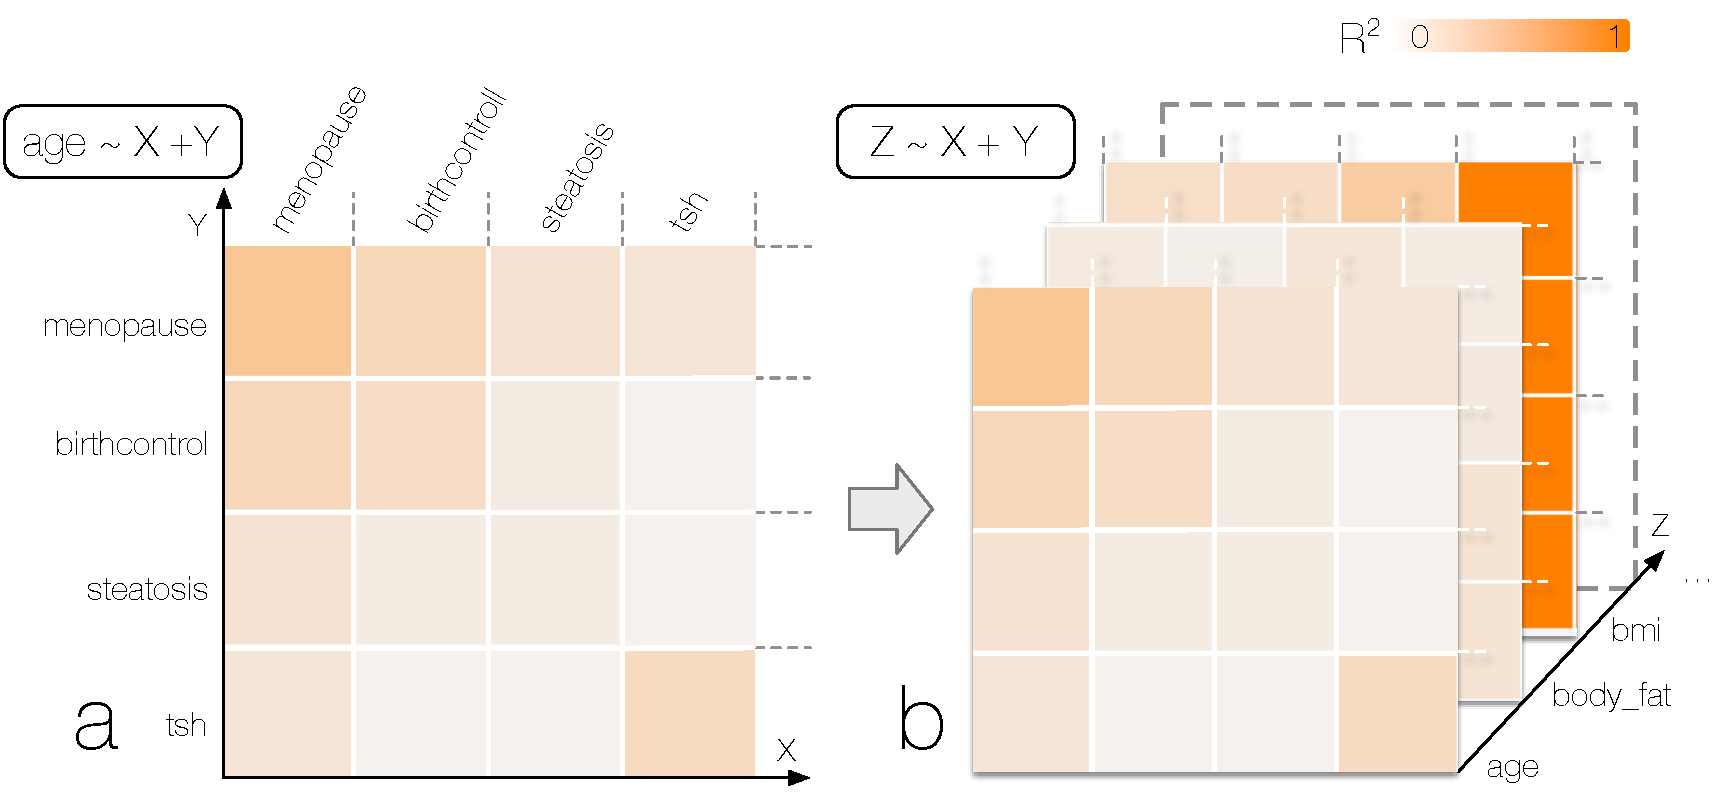
\includegraphics[width=1.0\linewidth]{figures/heat_map}
 \caption{
 (a) Overview visualization using a 2D heat map of the formula $Z \sim X + Y$, where $Z$ assumes the feature $age$.
 %%
 The $R^2$ metrics extracted from the regression model are mapped to color saturation (a saturated color indicates a strong correlation).
 %%
 (b) Now, $Z$ is set to all features $n$ and yields $n$ 2D heat maps.
 %%
 These represent the slices in our \emph{3D Regression Heat Map}.
 %%
 The metric describing the regression model of each slice voxel is mapped on opacity in the 3D view later on, reducing the occlusion of other values.
 }
  \label{fig:Heat_Map}
\end{figure}
%%
\noindent The goal of an overview visualization is to provide a comprehensive view on the data (raw or using descriptive metrics \cite{Bertini}), which is easy to understand.
%%
As described in our previous work \cite{Klemm2014VIS}, correlation values scaled between 0 (no correlation) and 1 (perfect correlation) can be encoded with color in a 2D heat map.
%%
Regression models are more complex, having many associated describing metrics.
%%
For the \emph{3D Regression Heat Map} analysis we are interested in the quality-of-fit of the resulting model.
%%
This allows to infer the predictive quality of the independent features included in the model.
%%
The $R^2$ \add{, adjusted $R^2$ and AIC} value are metrics allowing for this kind of assessment (recall Sect.~\ref{sec:RegressionAnalysis}).
%%
% \add{
% %%
% Users with in-depth knowledge about regression models are given the option to render the \emph{3D Regression Heat Map} using other descriptive features presented in \ref{sec:RegressionAnalysis}.
% %%
% Therefore, these experts can investigate the cube with emphasis on specific aspects of the model.
% %%
% To avoid shutting out users unfamiliar with these metrics, the \emph{3D Regression Heat Map} is set per default to show $R^2$ values.
% }
%%
\paragraph{2D (slice) view.}
%%
Since $R^2$ is scaled between $[0, 1]$, it allows for comparison \emph{between} regression models.
%%
We can apply the same 2D heat map by translating the $R^2$ values to \emph{color saturation} (Fig.~\ref{fig:Heat_Map}a).
%%
This encodes a 2D regression square for dynamic variables $X$ and $Y$ (e.g., $Age \sim X + Y$).
%%
\design{
%%
Based on expert feedback on early versions of this view, the amount of features used to compare regression models was extended.
%%
Therefore, these experts can investigate the heat map with emphasis on specific aspects of the model.
%%
}
%%
\add{
%%
$Adjusted$ $R^2$ can be represented in the same way, since they share the scale.
%%
$AIC$ values have to be normalized in order to map them onto color saturation.
%%
%The resulting scale may be distort by outliers, which requires facilities for allowing the user to select scale ranges.
The resulting scale may be distorted by outliers derived from poor regression models.
%%
To tackle this problem, we provide a slider input, which maps the transfer function of the metric to color saturation based on user-selected ranges.
%%
Outliers can be cut off to emphasize ranges of interest.
%%
Small $AIC$ values indicate a good model.
%%
Hence, we inverted the transfer function mapping it to color, mapping low $AIC$ features to saturated colors.
%%
}
\design{
%%
To include users unfamiliar with these metrics, the \emph{Regression Heat Map} is set per default to show $R^2$ values.
%To avoid shutting out users unfamiliar with these metrics, the \emph{Regression Heat Map} is set per default to show $R^2$ values.
%%
}

\paragraph{3D view.}
%%
Introducing $Z$ creates a 3D heat map (Fig.~\ref{fig:Heat_Map}b).
%%
\add{The selected metric (per default set to $R^2$)} of each heat map entry (\emph{voxel}) are mapped to opacity to reduce the overlap.
%%
\magenta{Object size is not used to encode information because it would result in a cluttered view.}
%%
\design{
%%
Epidemiologists argued, that the visualization of descriptive metrics derived from different regression methods (e.g., $Z \sim X + Y$) is misleading, as they can be compared relatively, but not in precise numbers.
%%
Therefore, we decided to map metrics of different regression methods on distinct colors (i.e., orange for linear regression and blue for logistic regression).
%%
}
%%
%The visualization of descriptive metrics derived from different 3D Regression Heat Maps (e.g., $Z \sim X + Y$) is misleading, as they can be compared relatively, but not in precise numbers.
%%
%Therefore, the $R^2$ results of different regression methods are encoded using different colors (i.e., orange for linear regression and blue for logistic regression).
%%
Thus, the visualization can be easily extended using other regression types.
%%
For \emph{3D Regression Heat Maps} with a fixed target feature, e.g., $Cancer \sim X + Y + Z$, no such encodings are required and the $z$ dimension can be compared directly.
%%
\magenta{
As mentioned previously, the feature reduction using the CFS algorithm potentially removes important features. %important to the domain expert.
%%
The $z$ dimension of the visualization contains \emph{all} features of the data set, allowing to assess their influence.
%%
The $x$ and $y$ dimensions are restricted to the features extracted from the CFS algorithm.
}
%%
\\\\
%%
Our goal is to create an overview visualization for a data set.
%%
We also want to incorporate expert knowledge into the visualization by adapting the underlying formulas.
%%
These two approaches do not exclude each other, they rather underline the difference in purpose of the chosen formula.
%%
The different analysis approaches require different starting points using the \emph{3D Regression Heat Map}.

\subsection{Analysis Workflow} \label{sec:Workflow}
%%
% \begin{figure}[htb]
%  \centering
%  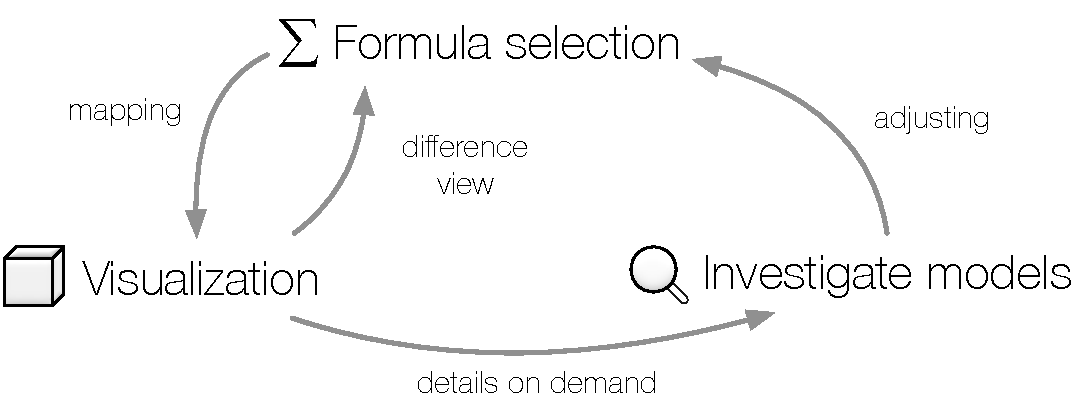
\includegraphics[width=1.0\linewidth]{figures/workflow}
%  \caption{
%  Different workflow types using the \emph{3D Regression Heat Map}.
%  %%
%  [\textbf{1.AF}] The workflow starts by declaring a formula to specify a hypothesis, or to use a predefined formula for a hypothesis-free analysis.
%  %%
%  [\textbf{2.SI}] The \emph{3D Regression Heat Map} is then visualized.
%  %%
%  The user has the option to either adjust the formula, adjust the transfer function or to derive details-on-demand on models.
%  %%
%  [\textbf{3.ZF}] Insights into the data yield either an adjustment of the current formula or a selection of a difference view.
%  %%
%  The latter is used to compare \emph{3D Regression Heat Maps}.
%  %%
%  [\textbf{4.DD}] Details about features using the 2D heat map representation yield insights and hypotheses about feature relations.
%  }
%   \label{fig:Workflow}
% \end{figure}
%%
\noindent Our \emph{3D Regression Heat Map} model is well suited for different workflow analysis techniques, based on the Visual Analytics (VA) Mantra of Keim et al.~\cite{Keim}:

\textbf{Analyze first} [\textbf{1.AF}]. Choosing an initial regression formula triggers the \emph{3D Regression Heat Map} calculation, filtering the dimensions of the dependent feature through the CFS algorithm.

\textbf{Show the important} [\textbf{2.SI}]. The 3D visualization acts as an overview over the whole data set.
%%
Here, regression models with large regression metric values can be spotted fast, steering the user's attention to the respective slice.

\textbf{Zoom, filter and analyze further} [\textbf{3.ZF}]. The slices of interest can then be analyzed using the 2D heat map of the slice.

\textbf{Details-on-demand} [\textbf{4.DD}]. Precise information about the individual regression models (coefficients, associated confidence intervals and p-values) can be retrieved based on the data point representatives (e.g. in a hover modal on a currently selected data point).
\\\\
We use the squared bracket abbreviation for each step to denote the affiliation to the system design section later on.
%%
%As shown in Fig.~\ref{fig:Workflow}, the workflow is highly iterative.
The workflow is highly iterative.
%%
Observations in the 2D heat map or simply the CFS-based features can trigger new analyses by adjusting the underlying regression formulas.
%%
This can be carried out either to refine the current formula based on observations, or to create a new \emph{3D Regression Heat Map} for a difference view.
%%
\paragraph{Hypothesis-free and hypothesis-based analysis.}
%%
\design{
%%
Early analysis sessions yielded two approaches of analyzing the data.
%%
The classic approach is \emph{hypothesis-based}, where the expert already knows the data and potential associations (e.g. reproducing knowledge about hepatic steatosis risk factors based on known risk factors).
%%
The \emph{hypothesis-free} analysis allows to derive new insights, such as identifying confounding features or potential targets (e.g. deriving risk factors for breast cancer associated features).
%%
}
%%
%Input formulas reflect \emph{hypotheses} about the data.
\emph{Hypotheses} about the data are reflected using input formulas.
%%
Using the operators, dynamic variables and dataset features, many different assumptions can be expressed.
%%
To support the \emph{hypothesis-free} analysis, we provide a default formula:

$Z \sim X + Y$.
%%
It represents all possible combinations of two independent features w.r.t. all features in the data set, since we do not know which features are of interest.
%%
Each slice represents a different target feature.
%%
It is therefore suitable for an exploratory analysis.

Hypotheses about the data are easily built up by relating dynamic variables with the regression operators.
%%
Furthermore, static features can be added for each regression formula.
%%
Here are a few examples:

%% TODO: First example can be cut if needed
$Cancer \sim X + Y + Z$ is the formulation of a hypothesis, where the specific feature \textit{Cancer} is analyzed.
%%
All combinations of three independent features with the target are analyzed through this \emph{3D Regression Heat Map}.

$Cancer \sim X + Y + Z + feature_1:feature_2$ encodes more assumptions.
%%
This formula models the hypothesis of an interaction between $feature_1$ and $feature_2$ (denoted with `$:$') being relevant for the target feature, but it is not clear how other feature combinations influence the result.
%%
Therefore, this interaction is incorporated for all $X$, $Y$ and $Z$ values as independent features.
%%

$Cancer \sim X + Y + Z$ subtracted with the regression metric from $Cancer \sim Age$ excludes the confounding effect that age has in view of the target $Cancer$ feature.
%%
This is achieved through \emph{3D Regression Heat Map} comparison.
%%

\paragraph{3D Regression Heat Map comparison.}
\design{
%%
Comparisons were introduced later in the project.
%%
Epidemiologists with focus on statistics pointed out, that comparing outcomes of different formulas is suitable for removing the effect of possible confounding features.
%%
}
%%
\emph{3D Regression Heat Maps} can be compared by creating difference views.
%%
One formula acts as reference.
%%
The absolute difference in the regression metric values with the second formula is calculated. %yielding the difference containing only the differences between the two formulas.
%%
For example, it can be utilized for comparing the influence of a single feature on the complete result (e.g., $Z \sim X + Y$ and $Z \sim X + Y + Income$).

\section{System Design} \label{sec:SystemDesign}
\begin{figure}[htb]
 \centering
 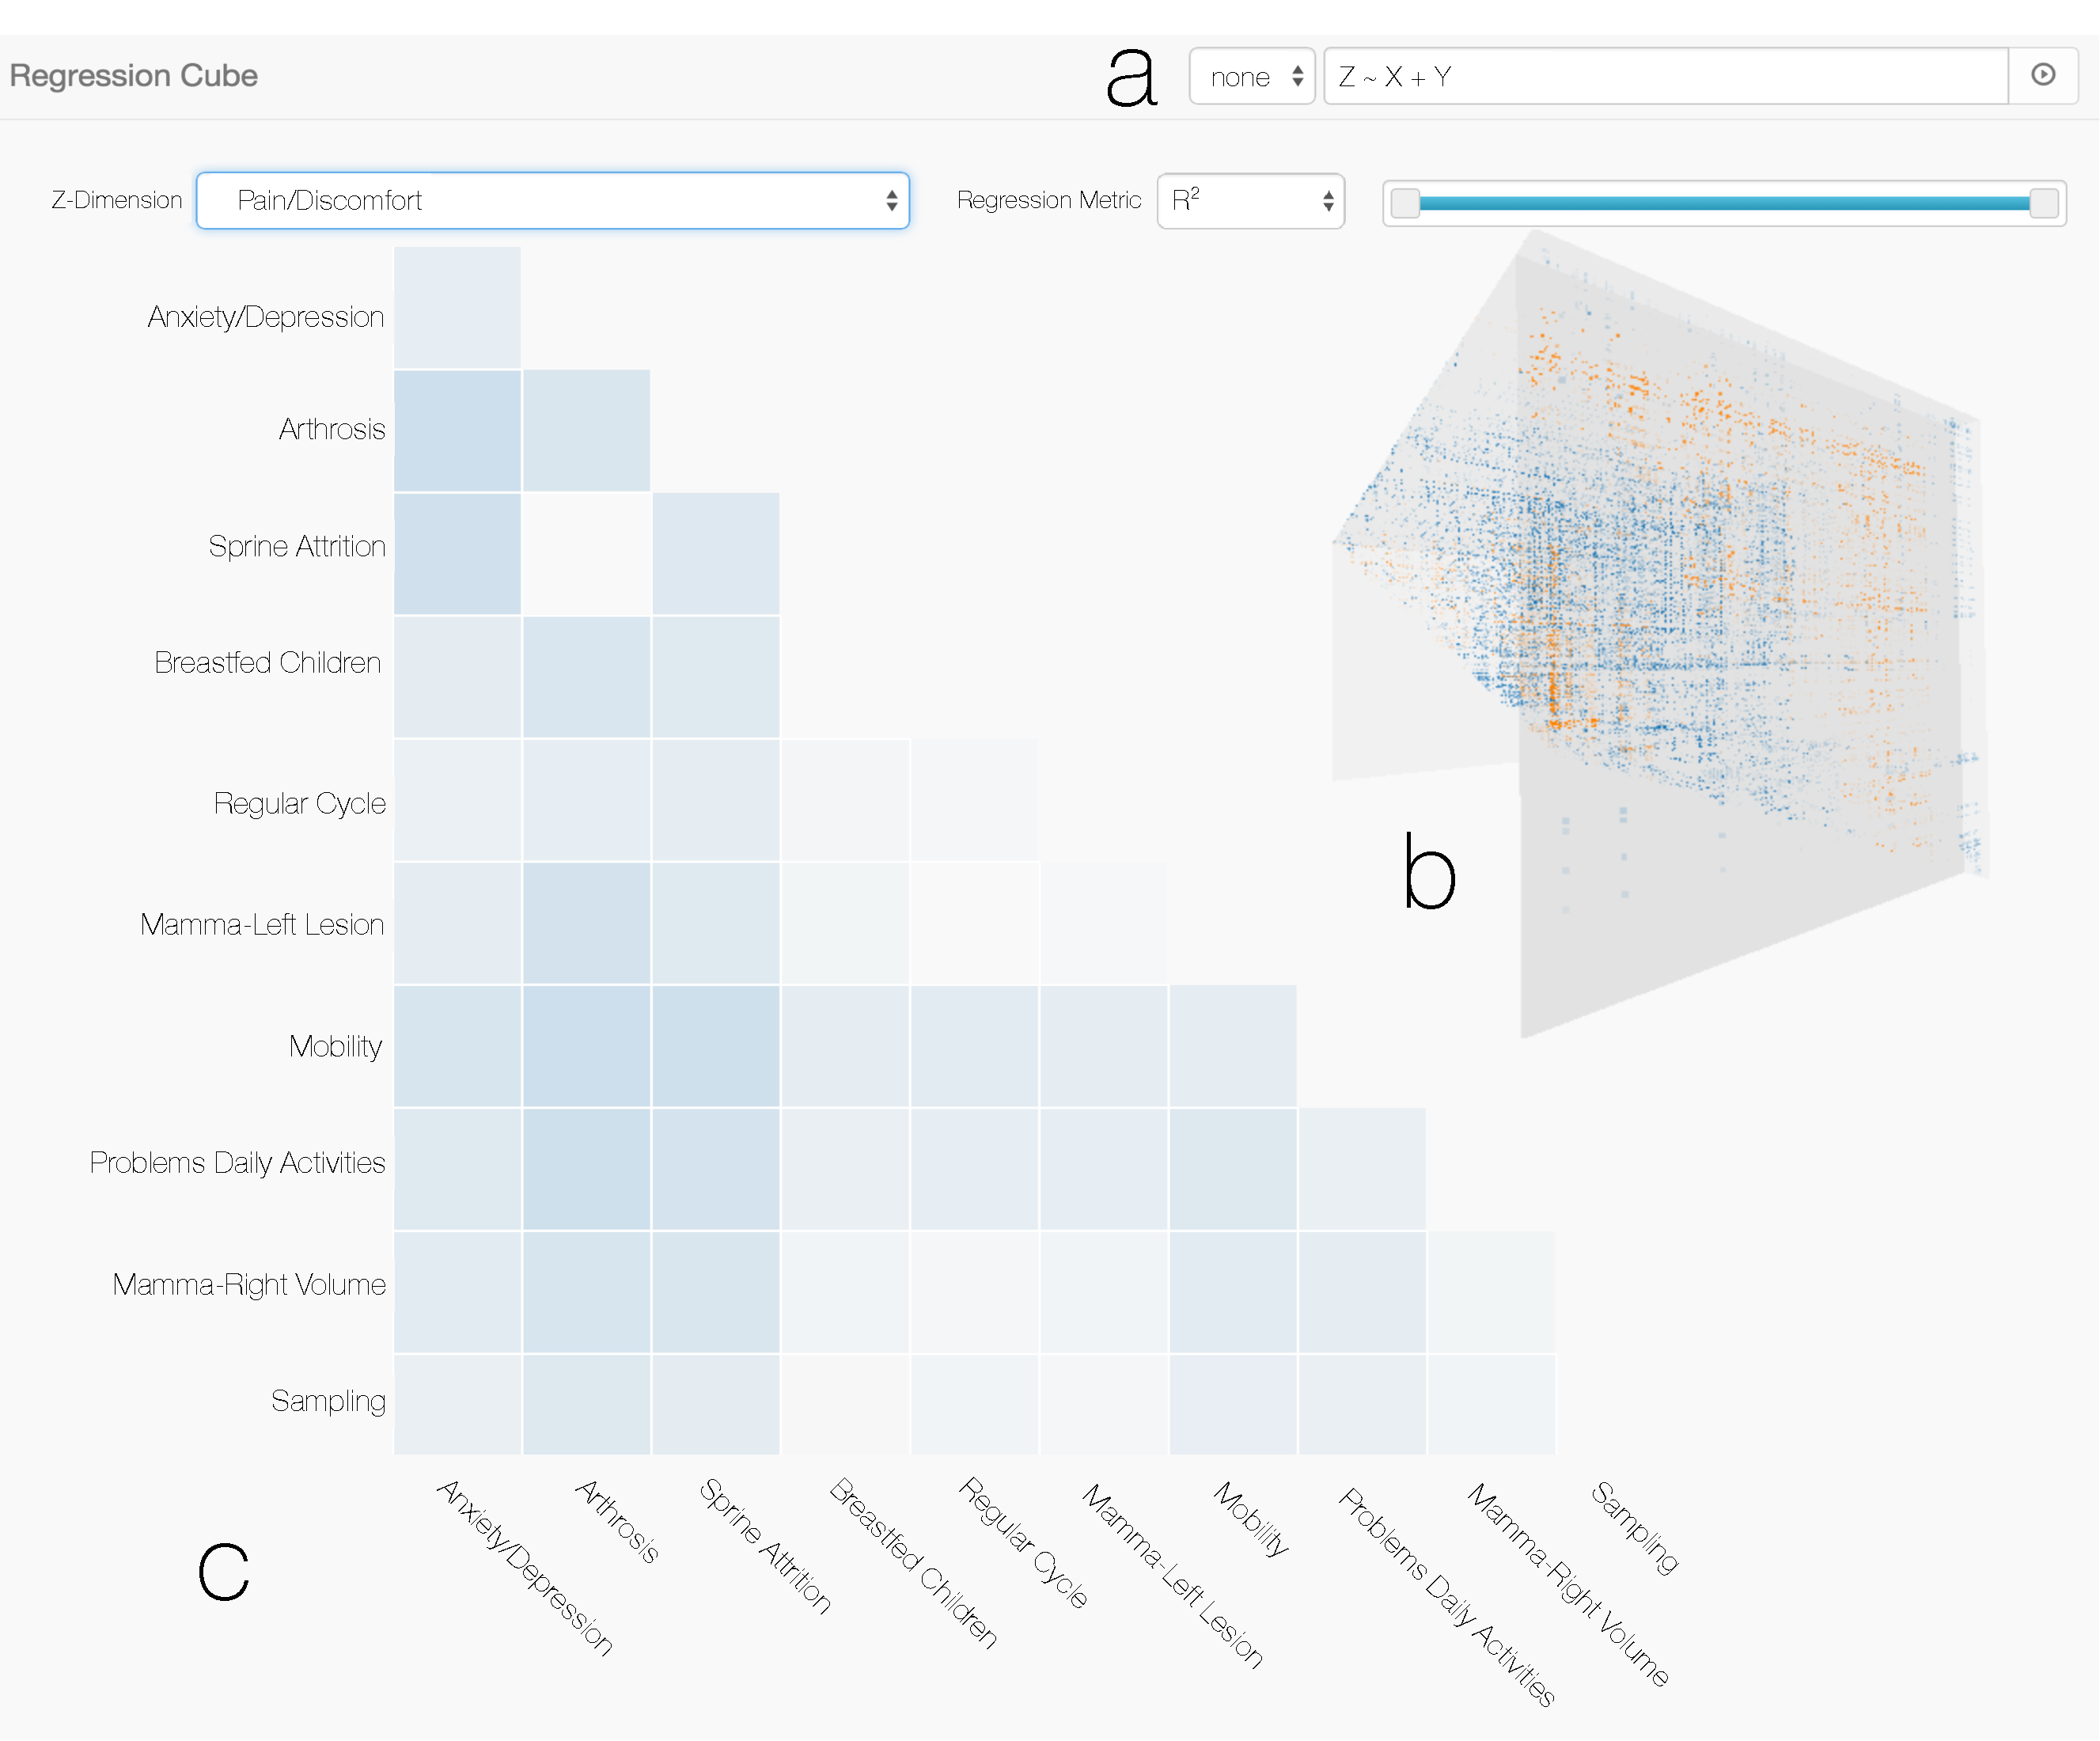
\includegraphics[width=1.0\linewidth]{figures/system}
 \caption{
 %%
 Breast density data set loaded into our prototype.
 %%
 (a) Using the formula input, the user specifies the dependent feature and calculation rules.
 %%
 (b) 3D heat map, showing values above the matrix diagonal as overview.
 %%
 The values of the currently selected slice are mirrored and represented as orange data points on the slicing plane.
 %%
 (c) 2D heat map of the selected slice for feature \emph{Pain/Discomfort}.
 %%
 }
  \label{fig:System}
\end{figure}
%%
%Albeit our focus on epidemiological data sets, we designed our system to be open with open formats as input interfaces .
%%
\noindent We designed our system to be openly accessible and easy to use.
%%
With open formats as input interfaces, the application can be extended to non-epidemiological data sets.
%%
The focus lies on creating an overview visualization and gaining insight into relationships of the data, which triggers further analyses with other (statistical) tools.
%%
\magenta{This is, however, out of the scope of this work.}
%%
Therefore, the system has to be intuitive and comprehensive in order to be adapted by domain experts.

%%
\design{
%A key requirement was little set up time to reduce the effort on the domain expert side, as they are mostly practicing clinicians with small time-frames for epidemiological research.
Using web-based technologies offers various advantages w.r.t. the collaboration with epidemiologists.
%%
They usually have little time to wrangle software.
%%
A web-based approach has no set-up time besides loading up the data set and can be carried out with any computer connected with the web.
%%
We can even implement small changes based on feedback of domain experts directly during analysis sessions. %and just requires a page reload.
%%
By providing a service using a website it has a much larger chance of being tested and potentially adapted by a broad user base.
%%
}
%Design choices and spaces are restricted by the underlying technologies and devices.
%%
%Therefore, the exchange of data and methods using web-based technologies offers many advantages.
%%
%There is no set-up time involved and domain experts can use the methods from any computer connected with the web.
%%
Web technology is based on a client-server architecture.
%%
It allows for outsourcing computationally heavy tasks on server clusters and transferring results to the client device.
%%
\magenta{
%%
This architecture is also prone to security issues, such as the storage of confidential data, especially in the epidemiological context.
%%
Therefore, we have to incorporate technical measures to ensure a secure workflow.
%%
}
%%
%The design space spanned by web technologies is different to standard WIMP applications: right-click menus, modal windows and menu bars are no established user interface components in this context.
%%
%Therefore, we have to adapt our design respecting the conventions of web pages.
%%
\subsection{System Paradigm and Components}
%%
\design{
%%
%Epidemiologists have little time slots available for their research.
Epidemiologists will not adapt complex systems, which require substantial training and time. %to work with are not suitable. %for the task of deriving overview visualizations.
%%
%If the system is not easy to learn, it will not be adapted.
%%
}
%%
%The \emph{3D Regression Heat Map} design focuses on a clean appearance, reducing the amount of user interface elements as much as possible.
Therefore, the \emph{3D Regression Heat Map} design focuses on a clean appearance, reducing the amount of user interface elements as much as possible.
%%
This allows for a fast learning of the system.
%%
Our prototype consists of three components:
\begin{itemize}
	%%
	\item The \emph{file upload} section starting the analysis with providing a comma-separated value (CSV) file [1.AF].
	%%
	\item The \emph{Regression Heat Map visualization} consisting of the 2D heat map as well as a 3D representation of all regression models \add{with facilities to change the represented regression metric and its range} [2.SI].
	%%
	\item The \emph{formula editor} allows formula input w.r.t. a hypothesis or to conduct a \emph{hypothesis-free} analysis.
	%%
	It also allows to select a reference formula for creating difference models [1.AF, 3.ZF].
	%%
\end{itemize}
%%
\paragraph{File upload and classification [\textbf{1.AF}].}
%%
Popular analytics tools, such as WEKA \cite{WEKA}, owe part of their success to their support of open file types.
%%
To allow other users even outside the epidemiological application domain to access to our tool, we use standard ASCII-based CSV files.
%%
The first line in a CSV file represents all features (columns) of the data set.
%%
Each line after that represents one subject (row) and its feature manifestations.
%%
\magenta{Using a check box, the user can disable the CFS preprocessing step, which is useful for small data sets, where the user does not want to reduce the number of features.}

% \textbf{Encoding via CSV Files.}
% %%
% Encoding variable types in CSV files is not standardized.
% %%
% However, we need to ensure the correct variable type classification and have to enforce some basic standards.
% %%
% All categorical values have to be enclosed by quotation marks.
% %%
% Continuous variables are denoted as digits without enclosing quotation marks.
% %%
% Although this seems obvious, many cohort study data sets encode categorical features using ID values that are denoted in a data dictionary.
% %%
% Variables with only two manifestations are classified as dichotomous, leading to three possible data types: numerical, categorical and categorical/dichotomous.
% %%
% Missing values are denoted by using no character at all, a whitespace, or an empty quotation mark encapsulated string.

\textbf{Data security} issues are raised by uploading data into an online service such as our prototype.
%%
The use of epidemiological data is preceded by a detailed description of the analysis purpose and has to be approved by ethics committees.
%%
Preventive steps have to be taken to restrict access to unauthorized subjects.
%%
We calculate a SHA-256 hash to derive the data set name using the data contents and disable directory listings on the web server to avoid data set downloads.
%%
Data sets are deleted from the server after closing a session.

\paragraph{Formula editor [\textbf{1.AF}, \textbf{3.ZF}].}
%%
After uploading the data, the user can specify a formula or use the default ($Z \sim X + Y$).
%%
Entering a formula is facilitated via text input.
%%
On formula input, a context panel displays all data set features as well as the available operators and their function.
%%
This allows to comprehend the function of the underlying formula for users without statistical background about regression analysis and its notation.
%%
Auto-completing input features also simplifies the approach and works as spell check of feature names.
%%

\textbf{Formula validation} is carried out directly on input.
%%
The text input containing the formula is marked using a red halo to indicate invalid input, which turns green for valid formulas.
%%
This prevents processing errors on the statistical processor back-end.
%%
Confirming a formula triggers the \emph{Regression Heat Map} \textbf{calculation}, which is preceded by determining all required formulas.
%%
These are then divided by the number of available statistical back-end processors, driving a \emph{cloud computing}-based approach.
%%
In theory, the calculation duration is reduced by a factor of $2$ by every statistical processor.
%%
In practice, data transmission and differences in machine specifications always influence the speed.

%%
\textbf{Difference heat maps} can be generated for each formula added to the system. %also adds it to the reference selection for a difference \emph{Regression Heat Map}.
Using a dropdown menu it can be selected as reference.
%%
Since all cells in the heat map are represented using regression metric values, the difference is the absolute difference of regression metric for each cell.
%%
\subsection{3D Regression Heat Map Visualization [2.SI].}
%%
The visualization and interaction with the \emph{3D Regression Heat Map} is the core of the prototype.
%%
Results from the statistical processors are uploaded into the visualization slice by slice.
%%
This allows the assessment of the data as soon as parts of the calculations are finished while the rest is still in progress.

\paragraph{Usage of a regression prism for information reduction.}
%%
Figure~\ref{fig:Heat_Map} shows that all values are mirrored along the diagonal of the 2D heat map matrix.
%%
This is due to the symmetry of basic regression operators.
%%
%$Z \sim X + Y$ produces the same result as $Z \sim Y + X$.
%%
Therefore, we can discard half of the results to reduce visual clutter and repetition, yielding a \emph{Regression Prism}.
%%
This opens up space for displaying additional information.
%%
Along the diagonal, $X$ and $Y$ represent the same feature, $Z \sim X + Y$ turns into $Z \sim X$ because the regression automatically ignores doublings.
%%
The diagonal therefore acts as reference on how strong the correlation for the given row (or column) feature is.

\paragraph{Selecting and scaling the descriptive regression metric.}
\design{
%%
The feedback made apparent that other features are of interest for analyzing regression models too.
%%
Hence, UI elements for controlling them were introduced.
%%
}
\add{
%%
The descriptive metric shown in the 2D/3D view can be selected using a dropdown menu.
%%
The default selection is $R^2$.
%%
$AIC$ displays model quality.
%%
\emph{Adjusted} $R^2$ values are only available for linear regression.
%%
Logistic regression results are represented via $R^2$ values in this mode.
%%
As they are visually distinguished using color, confusions are avoided.
%%
The transfer function of the color intensity (2D) and opacity (3D) can be adapted using a slider input.
%%
This additionally allows to filter models with desired features, such as only very high $R^2$ values.
}

\paragraph{3D prism as data mini-map.}
\design{
%%
In early prototype versions, the 3D prism acted as starting point for the data analysis without the implementation of a separate 2D view.
%%
Slices were shown using cutaway planes.
%%
This approach was not popular among epidemiologists, because the complexity of the visualization overwhelmed them. %did not like the combination of 3D interaction and slicing with representatives.
%%
}
%%
The \emph{3D Regression Heat Map} representation \design{was redesigned to} act as an overview over the whole data set.
%%
%Its purpose is not to derive detailed information about data points.
%%
It serves as a function similar to a mini-map, guiding the attention to points of interest in the data.
%%
It also gives context information about adjacent data values when using the 2D heat map.
%%
\design{The distinction between overview and details-on-demand using two different representations was well received with our domain experts.}
%%
The displayed prism shows values above the matrix diagonal.
%%
For formulas with a dynamic target feature (e.g. exploratory analysis using $Z \sim X + Y$), the color encodes the absolute regression metric values (Fig.~\ref{fig:System}b).
%%
Applying this strategy to a formula containing a static target (e.g. $Cancer \sim X + Y + Z$) yields many occlusions, since the CFS algorithm creates the same feature space for every slice.
%%
For such formulas, the 3D view encodes every data element as absolute difference between its regression metric values and the global mean along the z-axis.
%%
This highlights slices with unusually low or high results (Fig.~\ref{fig:Application}).
%%
\magenta{Variables are ordered the same way in the 2D and 3D heat map to preserve the mental model and make them visually analogous.}

\paragraph{Tackling the disadvantages of 3D information visualization.}
%%
3D information visualizations are criticized for introducing occlusions and interaction problems.
%%
These are often not balanced out by the advantages of using the third dimension for visual mapping.
%%
We aim to minimize these problems.
%%
The regression metric (e.g. $R^2$) values are mapped on data point opacity, highlighting large values in the prism, which guides the focus to the respective slices.
%%
The visualization is sparse, since the majority of regression models yield (depending on the data set and the chosen formula) low $R^2$ values.
%%
Also, the preceding correlation-based feature selection reduces the information space significantly, leading to sparse heat maps.
%%
Overlapping is still an issue, but greatly reduced in its effect to the visualization readability.
%%

%% INTERACTION
Transformation of the 3D heat map is restricted to the y-axis (horizontal only), preserving the mental map to position individual features.
%%
The 3D heat map is always oriented according to the 2D representation, allowing for an easy mental combination of them.
%%
Allowing more degrees of freedom was confusing to our users and also did not add value to the visualization.
%%
%Also we provide a zoom functionality using the mouse wheel input.
%%
\paragraph{3D heat map slice selection [\textbf{3.ZF}].}
%%
In order to \emph{Zoom, Filter and Analyze Further}, the user has to navigate to different slices of interest.
%%
We propose two ways to achieve this.

%\begin{itemize}
	%\item
	\textbf{We apply the slicing metaphor from 3D volume data.}
	%%
	In medical volume renderings, slicing views are common to view details on a selected plane in the scene.
	%%
	We employ this technique for selecting 3D heat map slices (e.g., by moving a plane via vertical mouse input while pressing the right mouse button).
	%%
	We, however, still display the whole 3D object instead of cutting away information. %down to the slice position.
	%%
	\design{Early prototypes only provided this method to select a slice of interest, which was inefficient when the user was looking for a specific slice.
	%%
	Hence, an additional method was implemented.
	%%
	}
	%%
	%\item

	\textbf{Selecting the slice using a dropdown menu} containing the feature names provides fast access to plane selections when the user already knows the slices of interest.
	%%
%\end{itemize}
%%
The currently selected slice is displayed as a semi-transparent gray plane.
%%
\design{
Early prototypes rendered the whole \emph{3D Regression Heat Map}, which made it hard to assess the position of the plane.
%%
%Since the regression metrics are mirrored along the diagonal, we decided to use this space to support better identification of the current slice.
Since the regression metrics are mirrored along the diagonal, the space available from visualizing only the prism generated from the upper half of the heat map diagonal is used to display the 2D heat map of the currently selected plane.
}
%%
The \magenta{regression metric values} are projected on this plane to provide an overlapping-free view.
%%
This allows for a easier to identify the current slice.
%%
\paragraph{2D heat map slice visualization [\textbf{4.DD}].}
%%
The 2D heat map (Fig.~\ref{fig:System}c) shows all values below the matrix diagonal of the current slice.
%%
It creates an optical equivalence with the 3D heat map.
%%
To reduce visual clutter, the 2D view only shows dimensions, which are retrieved through the correlation-based feature selection.
%%
The free space above the matrix diagonal is used to display the 3D heat map.
%%

The purpose of this view is the detailed assessment of the underlying regression models.
%%
By hovering over a data entry in the plot, a tooltip displays detailed information about a model's coefficients, associated $p$ values, confidence intervals \add{f-scores and AIC values}.
%%
\add{
%%
It also contains a scatter plot of the \emph{model residuals}, which shows the difference between the observed data points with the fitted values.
%%
Epidemiologists use such plots to validate models w.r.t. the model assumptions, such as homogeneity, normality, and independence \cite{GraphicModelAssessment}.
}

\section{Implementation} \label{implementation}
\begin{figure}[htb]
 \centering
 \includegraphics[width=1.0\linewidth]{figures/implementation}
 \caption{
 The front-end (left) is realized with \texttt{HTML5}/\texttt{CSS3}/\texttt{Javascript} and different Javascript libraries, such as \href{https://www.angularjs.org/}{\texttt{Angular.js}}, \href{http://threejs.org}{\texttt{Threejs}} and \href{http://d3js.org/}{\texttt{D3.js}}.
 %%
 The web-server (right) is written using \href{http://nodejs.org}{\texttt{Node.js}} and hosted on \href{https://www.heroku.com/}{\texttt{Heroku}}.
 %%
 \href{http://r-project.org}{\texttt{R}} and \href{https://www.opencpu.org/}{\texttt{OpenCPU}} constitute the statistical back-end (top) to compute the \emph{3D Regression Heat Maps}.
 %%
 Additional statistical back-ends can be attached to the system to decrease the computation time.
 %%
 }
  \label{fig:Implementation}
\end{figure}
%%
\noindent We rely on web-based technologies for our prototype.
%%
%The ongoing transition of open-science software into the web spawned numerous projects, making state-of-the-art algorithms available in this domain.
%%
%\paragraph{Front-End.}
%%
The front-end is created using \texttt{HTML5}, \texttt{CSS3} and \texttt{Javascript}.
%%
%\texttt{Angular.js}\footnote{Open Source; Maintained by Google, \href{https://www.angularjs.org/}{\texttt{angularjs.org}}} abstracts web application into models and views, allowing for a responsive way to combine \texttt{HTML} and \texttt{Javascript}.
\href{https://www.angularjs.org/}{\texttt{Angular.js}} abstracts web application into models and views, allowing for a responsive way to combine \texttt{HTML} and \texttt{Javascript}.
%%
It is easily expandable by forcing developers to write modularized code.
%It forces developers to write modularized code, which makes the components easier expandable. %while keeping the code maintainable by including unit tests.
%%
%The page layout is handled using \texttt{Twitter Bootstrap}\footnote{Open Source; Maintained by Twitter, \href{http://getbootstrap.com}{\texttt{getbootstrap.com}}}, which also provides a rich set of user interface elements.
\href{http://getbootstrap.com}{\texttt{Twitter Bootstrap}} handles the page layout and provides a rich set of user interface elements.
%%
The 2D heat map is implemented using the \href{http://d3js.org/}{\texttt{D3.js}}~\cite{D3} information visualization library.
%%
It provides fast and easy methods for binding data to graphical elements.
%%
%The 3D plot is created using the WebGL-based \texttt{Threejs}\footnote{Open Source; Originally developed by R. Cabello, \href{http://threejs.org}{\texttt{threejs.org}}} library.
The 3D plot is created using the WebGL-based \href{http://threejs.org}{\texttt{Threejs}} library.
%%
% We experimented with different ways for achieving the cube representation, including volume rendering, cube primitives for each data point and shader-based solutions.
% %%
% Open source volume rendering methods are available but do not satisfy our requirements.
% %%
% Creating a cube primitive for each data point resulted in non-interactive frame-rates for data sets larger than 30 features (creating 30$^3$ cube primitives).
% %%
% Therefore, we decided to use a shader-based solution by rendering the cube as a sprite-based particle system, allowing to customize color and opacity of every data point.
% %%
% It also is the fastest solution that we tested.

%\paragraph{Back-End.}
Two server structures serve as back-end.
%%
%The web-server is written in \texttt{Javascript} using \texttt{Node.js}\footnote{Open Source; Maintained by Joyent Inc, \href{http://nodejs.org}{\texttt{nodejs.org}}}, running on Googles V8 Javascript runtime environment.
The web-server is written in \texttt{Javascript} using \href{http://nodejs.org}{\texttt{Node.js}}, running on Googles V8 Javascript runtime environment.
%%
%It is hosted on \texttt{Heroku}\footnote{Owned by Salesforce.com, \href{https://www.heroku.com/}{\texttt{heroku.com}}}, a cloud application platform.
It is hosted on \href{https://www.heroku.com/}{\texttt{Heroku}}, a cloud application platform.
%%
The statistical computations are performed on the second structure.
%%
%They rely on the statistical programming language \texttt{R}.\footnote{Open Source; \href{http://r-project.org}{\texttt{r-project.org}}}
They rely on the statistical programming language \href{http://r-project.org}{\texttt{R}}.
%%
It is widely adopted in the statistical analysis community, yielding a rich support of state-of-the-art statistics algorithms as well newly published methods.
%%
\href{https://www.opencpu.org/}{\texttt{OpenCPU}} is an \href{http://r-project.org}{\texttt{R}} package and provides an API for accessing it via HTTP calls \cite{Ooms}.
%%
This way, any computer, which runs \href{http://r-project.org}{\texttt{R}} can be turned into a statistical processor for our project.
%%
% The back-end functions necessary for all cube calculations are provided via an \texttt{R} package.
% %%
% It uses multi-core optimization to use all machine CPUs to speed up the calculation process.
% %%
% The server workload balances are managed by the front-end code.

%\paragraph{Access and Source.}
%%
A running instance of the \emph{3D Regression Heat Map} prototype can be found under \href{http://regressionheatmap.herokuapp.com/}{\texttt{regressionheatmap.herokuapp.com}}.
%%
The source for the prototype is freely available at \texttt{Github}.\footnote{\texttt{R}-based back-end: \href{https://github.com/paulklemm/regression-heatmap-r-package}{\\\texttt{github.com/paulklemm/regression-heatmap-r-package}}}$^{,}$\footnote{Front-End and Node.js Webserver: \href{https://github.com/paulklemm/regression-heatmap-prototype}{\texttt{\\github.com/paulklemm/regression-heatmap-prototype}}}
%%
Instructions and code to setup running the statistical back-end through a \href{http://www.ubuntu.com/}{\texttt{Ubuntu}} server using \href{https://www.opencpu.org/}{\texttt{OpenCPU}} are included in the repository.
%%
The front-end can be deployed using \href{https://www.heroku.com/}{\texttt{Heroku}} by cloning the repository into a Heroku app.
%%
\section{Application} \label{application}
%%
\begin{figure*}[htb]
 \centering
 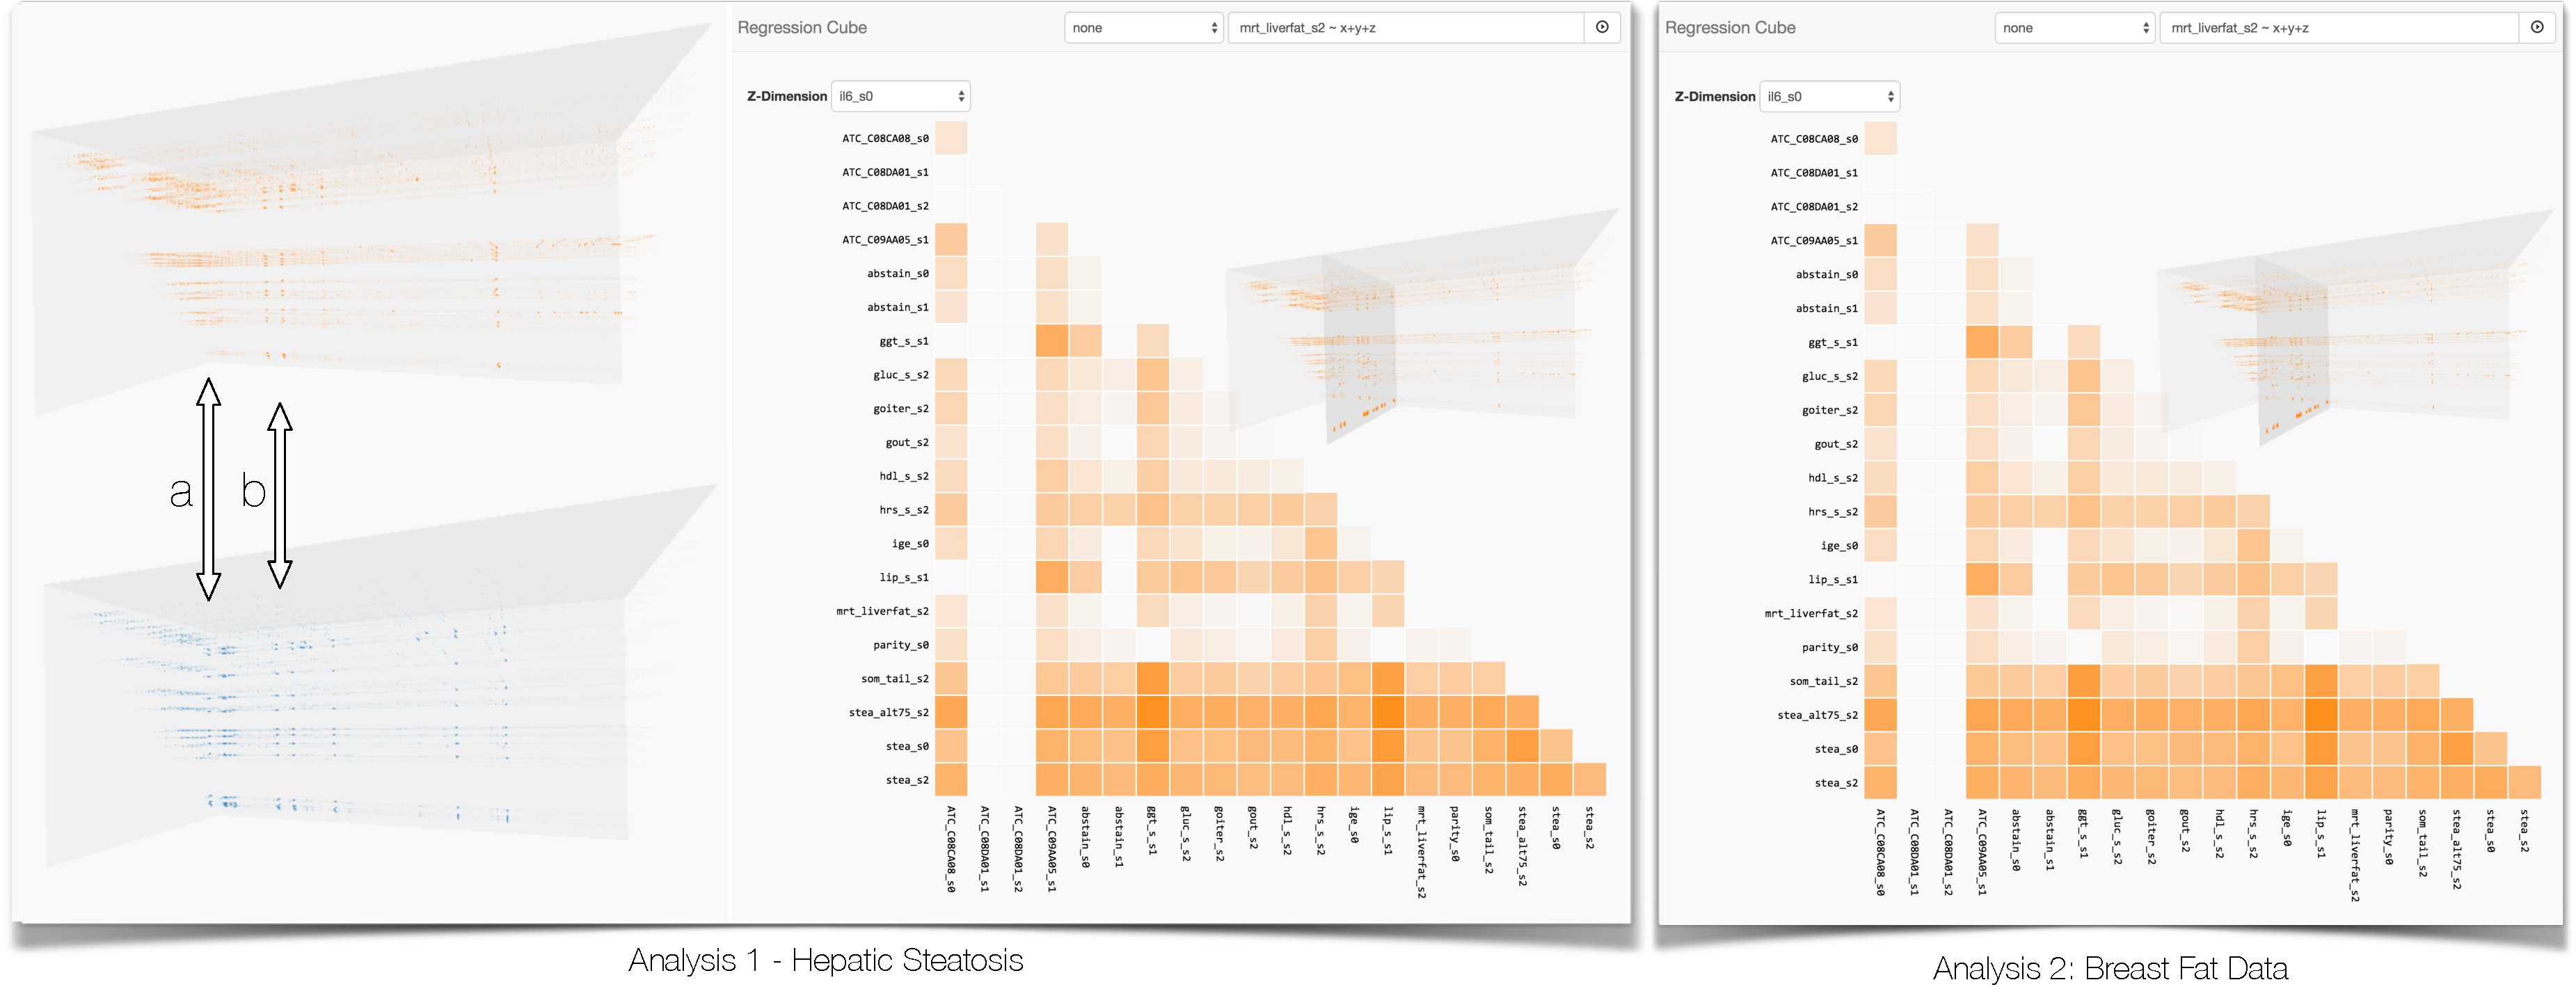
\includegraphics[width=1.0\linewidth]{figures/application}
 \caption{
 The analysis of the numerical and dichotomized target feature depicting liver fat values yields similar results (left).
 %%
 In (a), hotspots for somatometrical features with high correlations were found.
 %%
 High correlations were also found for features depicting \emph{hepatic steatosis} (b).
 %%
 A high correlation between \emph{Interleukin-6}, \emph{hepatic steatosis}, \emph{GGT} and \emph{Lipase} (highlighted using arrows) was revealed during the analysis using the 2D heat map.
 %%
 The hypothesis-free analysis of the breast density data set (right) w.r.t. the \emph{parenchyma tissue percentage} of the breast displays correlations between \emph{age}, \emph{body fat}, \emph{hip circumference} as well as \emph{menstrual period}.
 }
  \label{fig:Application}
\end{figure*}
%%
In this section, we describe the application of the \emph{3D Regression Heat Map} to two epidemiological data sets.
%%
The hepatic steatosis data set was analyzed using data mining algorithms, yielding risk groups, which we now analyze further.
%%
We try to reproduce the prior results from the analysis as proof-of-concept of our method.
%%
The female breast density data set is the basis for an explorative analysis w.r.t. the influencing parameters of the breast cancer related parenchyma tissue ratio.
%%

Both data sets are unusual for epidemiological analysis regarding their feature extent.
%%
Usually, only a few features depicting a hypothesis are compiled into a data set to assess them using statistical tools.
%%
The herein used data sets comprise several hundred features.
%%
Our method focuses on data exploration and knowledge extraction and requires a wide scope of sociodemographic, medical and lifestyle features.
%%
\subsection{Participants, Setup and Procedure}
%%
The knowledge discovery capabilities of a system are difficult to measure.
%%
The \emph{Visual Data Analysis and Reasoning} (\emph{VDAR}) technique proposed by Lam et al.~\cite{Lam2012} is focused on the characterization of a systems' ability to generate hypotheses and explore the data in order to extract information.
%%
\emph{VDAR} can be carried out based on case studies using thinking-aloud techniques to comprehend the users reasoning and thought process.
%%
We employ \emph{VDAR} for analyzing our system.
%%
\paragraph{Participants, setup and procedure.}
%%
We conducted a web-based analysis by using an online-meeting software, which features voice chat as well as screen sharing.
%%
Starting an analysis using these techniques takes about 5-10 minutes of setup time.
%%
The sessions started with an initial overview of the system, showcasing its features and functionality.
%%
Afterwards, the experts use the system on their own computers.
%%
The screen-sharing function was still used to observe the actions of the expert.
%%
All sessions were video recorded to be processed later on.
%%
We conducted the analysis with three participants.
%%
\emph{KH}, a clinician (10 years of experience) with focus on epidemiological research, is the domain expert for the breast density data set.
%%
She is a radiologist, responsible for the SHIP-MRI acquisition and also responsible of the mammography analysis.
%%
The hepatic steatosis data set is analyzed by \emph{UN}, a data scientist responsible for prior analysis of the data.
%%
The third participant is \emph{TI}, a statistician with focus on epidemiology (8 years of experience) assesses the statistical reliability of the tool and the underlying methods without a focus on a specific data set.
%%
\subsection{The Hepatic Steatosis Data Set}
We employ the data set used by Niemann et al.~\cite{Niemann2014} to identify predictive features w.r.t. the reversible hepatic steatosis disorder.
%%
The dichotomous target feature is derived from the liver fat concentration measured using MRI scans.
%%
Liver fat concentrations of no more than 10\% are mapped to the `negative' class; values greater than 10\% are mapped to the `positive' class to indicate absence or presence of the disease.
%%
The data set contains labels for 578 participants. %for which the MRI data was available to that point.
%%
The MRI scans for each subject are only available in SHIP-2. %, so the target feature is only present the last study wave.

%%
Apart from the target feature, the data set contains 199 features, comprising sociodemographic features (gender, age), consumption behavior (e.g., alcohol and tobacco), laboratory data (e.g., sera concentrations), and two features depicting the liver ultrasound.
%%
The acquisition wave is denoted using the appendix; 85 features with appendix \emph{s0} denote their affiliation to SHIP-0 (first study moment), 50 features for \emph{s1} and 55 for \emph{s2}, alongside with 10 time-independent SNPs (DNA base pairs).
%%
Niemann et al.~\cite{Niemann2014} show different class distributions of liver fat concentrations of women and men.
%%
For women, an association between age and liver fat was identified.
%%
An appropriate cut-off value of 52 years, which is the approximately the entry age for the menopause was set, yielding the most homogeneous class distribution within the resulting subsets.
%%
Based on these observations, we perform our analysis on three populations: \emph{males}, \emph{females (all ages)} and \emph{females older than 52 years}.
%%
\subsection{The Breast Density Data Set}
%%
The breast density data set was compiled to find associations between the parenchyma tissue proportion in the female breast compared to other features in the data.
%%
Breast density is denoted as the ratio between parenchyma and cellular connective tissue and has been shown to be associated with breast cancer.
%%
Studies describe a four to five times increased risk of getting breast cancer for participants with a breast density above 50\% \cite{Mccormack2006}.

The data comprises 1,186 female subjects. %(368 from \texttt{SHIP-2}, 818 from \texttt{SHIP-TREND-0} cohort).
%%
It contains 231 features, holding information about somatometric features (e.g., body size and weight) consumption behavior, personal and medical history (e.g., occupation and prior diseases), women-specific features (e.g., number of born children and contraception type) as well as mammography features (e.g., fat content and parenchyma tissue proportion to volume).
%%
The latter were derived from MRI data for each subject, which was manually segmented by radiologists \cite{Hegenscheid2009, Ivanovska2014}.
%%

The data of each cohort was presented as individual \texttt{SPSS} files.
%%
All features related to the mammography attributes were stored in an additional file.
%%
We converted the \texttt{SPSS} data sets to CSV and used \texttt{R} to merge the data sets together using their ID.
%%
All features were renamed to be self-explaining, e.g., \emph{chro\_09a} is now denoted as \emph{Disease\_Osteoporosis}.
%%
This avoids the need of defining a separate data dictionary file for translating the feature names.
%%
\subsection{Case 1: Hypothesis-Driven Analysis of the Hepatic Steatosis Data Set}
%%
We refer to each analysis step with regard to its belonging in the VA-Mantra (recall Sec.~\ref{sec:Workflow}).
%%
The analysis goal was reproducing results with our visual analysis framework that are in accordance to the data mining-based results presented by Niemann et al.~\cite{Niemann2014}.
%%
Therefore, \emph{UN} started the [\textbf{1.AF}] step using the dichotomized MRI fat liver concentration and the formula $mrt\_liverfat\_s2 \sim X + Y + Z$ for \emph{male} subjects.
%%
The [\textbf{2.SI}] step using the 3D heat map locates hotspots at the end of the heat map (Fig.~\ref{fig:Application} left).
%%
The Zoom, Filter and Analyze Further Step [\textbf{3.ZF}] was realized by slicing through the 3D heat map using the mouse input to inspect the hotspots.
%%
Analyzing the 2D heat map [\textbf{4.DD}] revealed high correlations for somatometric features, hepatic steatosis indicator features as well as laboratory values, such as \emph{creatinine} (used as renal retention parameter) and \emph{uric acid} (used as gout and diabetes risk factors) magnitudes.
%%
Similar results were present for analyzing the \emph{female} groups.
%%
\emph{UN} could reproduce most results.
%%
Some features exhibit lower correlations, e.g., \emph{creatinine} magnitudes.
%%
A slight influence of \emph{age} on the target feature could be observed for women ($R^2$ of $0.09$ for females compared to $0.02$ for males).
%%
Relationships not described by Niemann et al.~\cite{Niemann2014} were found, such as enzymes indicating liver dysfunctions, e.g., \emph{aspartate aminotransferase}.
%
%%
Due to the difference between our regression model approach and the decision tree approach presented by Niemann et al.~\cite{Niemann2014}, a complete matching set of correlating features is not expected.
%%

%%
\paragraph{Analysis of non-discretized target feature.}
%%
Since our method can assess numerical target features, the analysis was conducted again for the non-dichotomized target using the same formula.
%%
The 3D heat map showed lower $R^2$ values in general.
%%
However, the analysis is now based on linear regression and the $R^2$ values cannot be compared directly.
%%
The correlation hotspots matched with the ones from the dichotomous target, but were generally lower ($R^2$ of $0.37$ for somatometric features as opposed to $0.58$).
%%
We assume that the bias introduced by dichotomizing the fat liver content enforces the findings of liver diseases, while using the numerical features is less expressive.

\paragraph{Interleukin-6 correlation with liver fat.}
%%
During the analysis, one hotspot was always observable in the [\textbf{2.SI}] and [\textbf{3.ZF}] steps, incorporating a high \emph{Interleukin-6} (\emph{IL-6}) correlation with liver fat values ($R^2$ of $0.8$, see Fig.~\ref{fig:Application}b).
%%
The correlation was high for both the dichotomized and continuous target feature.
%%
The literature described relations between \emph{IL-6} and liver cancer \cite{He2013} as well as chronic liver diseases \cite{Streetz2003}.
%%
For mice, strong effects of \emph{IL-6} with hepatic steatosis were described \cite{Hong2004}.
%%
The finding is subject of further analysis.
%%
\subsection{Case 2: Hypothesis-free Analysis of the Breast Density Data Set}
%%
The analysis aims to find relationships on the breast density data using mammography analysis features.
%%
Relationships between the share of parenchyma tissue on the overall breast volume are of high interest \cite{Mccormack2006}.
%%
The [\textbf{1.AF}] was started by \emph{KH} using the default formula for hypothesis-free analysis ($Z \sim X + Y$).
%%
At first, she was interested in correlations with the \emph{parenchyma tissue} percentage, which was selected through the drop-down for the z-axis [\textbf{2.SI}].
%%
She observed strong correlations with \emph{age}, \emph{body fat percentage}, \emph{hip} and \emph{waist circumference} as well as \emph{menstrual period} or \emph{pregnancy status} as expected (Fig.~\ref{fig:Application} right).
%%
Women with higher \emph{body fat} also have a larger \emph{breast density percentage}, which also correlates with other somatometric features.
%%
\emph{Age} is a strong influencing factor, as breast tissue and subsequently the parenchyma tissue degrades over time.
%%
\emph{KH} proceeded using [\textbf{3.ZF}] and [\textbf{4.DD}] to check for relationships for different target features, such as current \emph{hormone replacement therapy}, \emph{BI-RADS} (classification of the mammography findings) as well as different diseases, such as \emph{diabetes} or \emph{gout}.
%%
She observed relationships matching her expectations and expert knowledge.
%%
One unexpected relationship was observed between \emph{breast lesions} and \emph{menstruation cycle} w.r.t. \emph{spiral contraception} ($R^2$ of $0.77$).
%%
\emph{KH} proceeded with a detailed analysis of the parenchyma tissue.
%%
\paragraph{Detailed breast parenchyma analysis.}
%%
The analysis was conducted by calculating the formula $Parenchyma\_Percentage \sim X + Y + Z$ [\textbf{1.AF}].
%%
Using the 3D heat map, \emph{KH} observed several hotspots [\textbf{2.SI}].
%%
Navigating to them using the slicing facility of the 3D visualization [\textbf{3.ZF}] highlighted features of high influence, such as image-derived features, as \emph{glandular tissue density} and \emph{parenchyma segmentation} metrics.
%%
Also, strong correlations were observed in the \emph{diabetes} slice, confirming expectations of \emph{KH} w.r.t. its strong influence to the parenchyma tissue.
%%
A surprising finding was the strong correlations with \emph{kidney disorder} ($R^2$ values around $0.9$).
%%
The [\textbf{4.DD}] analysis, however, showed only 8 subjects with this disease.
%%
Too few subjects impose the risk of a biased finding.
%%
The correlation was noted and will be further investigated using an extensive data set.
%%
Lastly, \emph{KH} assessed the influence of contraception-related features, such as use of \emph{birth control pills} or the \emph{spiral}, but found no significant correlations with the parenchyma tissue.
%%
Other consumption behavior features, such as \emph{alcohol intake} also yield no elevated $R^2$ values.
%%
\emph{KH} remarked that these features are suspected to have an impact on the parenchyma tissue, but they are less reliable, since they are self-reported.
%%
\subsection{Further Feedback and Lessons Learned} \label{Lessons Learned}
%%
The presented method was well received among the domain experts.
%%
For the first time, they were able to derive an overview visualization custom-tailored to underlying assumptions.
%%
\emph{KH} noted the ease of use, which "\emph{converts data sets into a feasible form}".
%%
She highlighted the efficiency of combining fast target feature selection with visually highlighting interesting results, enabling rapid analysis cycles.
%%
To get nearly similar results, she had to spend hours using \texttt{SPSS} and potentially missed interesting hotspots during this process.
%%
\emph{TI} highlighted the ability to simultaneously analyze thousands of regression models while maintaining little time expenses for rating them.
%%

%%
\paragraph{Extracted hypotheses have to be investigated further.}
%%
We map results of complex statistical computations into comprehensive visualizations.
%%
Agreeing with \emph{TI}'s feedback, each finding and hypothesis has to be confirmed using a dedicated statistical analysis.
%%
An accompanying search for correlations potentially highlighting confounders can be carried out using our method.
%%
Statistical validation of an epidemiological result still has to be carried out by statisticians using their respective tools.
%%
\emph{TI} commented on the possibility of adding more regression types to model different correlation types.% to customize the cube even more.
%%

%%
\paragraph{Overview visualizations are preferred over black-box methods.}
%%
Explorative analysis based on the data gains importance in epidemiology with increasing data set complexity.
%%
Results from automatic `black-box' methods, such as data mining algorithms are more often obscure to the expert.
%%
Findings and hypotheses derived through overview visualizations, however, are met with more confidence, because the users actually observed the behavior themselves.
%%
The participation and steering of the analysis using human pattern detection and expert knowledge is preferred.
%%
Observing \emph{expected} correlations matching the expert knowledge strengthens the confidence in the method and, subsequently, in the hypotheses generated from unanticipated relationships.
%%

%%
\paragraph{Using non-discretized features reduces information bias.}
%%
Discretization reduces the information space and introduces bias into the data and is therefore avoided in epidemiological research whenever possible.
%%
In contrast to many data mining algorithms, our method allows to use the concurrent analysis of heterogeneous data types.
%%
Investigations of the hepatic steatosis data set with both numerical and dichotomized liver fat values showed comparable results. %but slightly differed when it comes to details.
%%
The overall explanatory power on the numerical feature was lower, supporting the hypothesis that the dichotomized target feature already models knowledge to bias the data w.r.t. the expected result.
%%

%%
\paragraph{Attention steering is crucial.}
%%
Important events have to be highlighted in overview visualizations to direct the user's attention to interesting parts of the data.
%%
Poor guidance potentially leads to overlooked relationships.
%%
We found the 3D heat map as supporting mini-map visualizations most useful for this purpose, e.g., for highlighting differences rather than displaying absolute values (Fig.~\ref{fig:Application}).
%%
\section{Summary and Outlook}
%%
We presented a technique for knowledge discovery in population study data sets with user-defined target features.
%%
Dimension reduction using the target restricts the analysis to the most important features.
%%
\emph{Hypothesis-free} analysis employs default regression models.
%%
Modeling expert knowledge using regression formulas allows for a \emph{hypothesis-based} investigation.
%%
A \emph{3D Regression Heat Map} allows to assess hotspots in the analysis by abstracting regression models using a quality-of-fit measure.
%%
These can then be analyzed further using the 2D plot for each 3D heat map slice.
%%
Details-on-demand for each model allow for a detailed assessment of regression models.
%%
We successfully applied the approach to find correlations in a hepatic steatosis as well as a breast density data set.
%%
The method was well received by our clinical partners, triggering detailed investigations of the findings.

\magenta{
%One limitation of the proposed method is that the regression metrics always only capture a part of the underlying model.
%%
%The analyst has to keep the aspects of the respective metric in mind to avoid false conclusions.
%%
The analysis is limited to three dynamic variables representing the \emph{3D Regression Heat Map} dimensions.
%%
Investigating more dynamic variables can be achieved by projecting the resulting high-dimensional space into a three-dimensional representation.
%%
This, however, increases the cognitive load and complexity of the analysis substantially and needs to be accompanied by techniques, which simplify this approach.
%%
Static features can be added using the formula input without increasing the complexity of the visualization.
}

As a next step, we want to introduce more regression types, which model different kinds of correlations.
%%
We also want to extend the 3D heat map to time-dependent data by expanding the difference heat map approach.
%%
We published all associated code and provide a freely accessible analysis platform open to heterogenous data types.
%%
We want to support opening up knowledge discovery to allow a diverse group of domain experts to derive insight into their data. %and support the notion of open science.
%%
\begin{small}
\acknowledgments{
%%
SHIP is part of the Community Medicine Research net of the University of Greifswald, Germany, which is funded by the Federal Ministry of Education and Research (grant no. 03ZIK012), the Ministry of Cultural Affairs as well as the Social Ministry of the Federal State of Mecklenburg-West Pomerania.
%%
Whole-body MR imaging was supported by a joint grant from Siemens Healthcare, Erlangen, Germany and the Federal State of Mecklenburg-Vorpommern.
%%
%The University of Greifswald is a member of the ‘Centre of Knowledge Interchange’ program of the Siemens AG.
%%
This work was supported by the DFG Priority Program 1335: Scalable Visual Analytics.
%%
Sylvia Gla{\ss}er and Kai Lawonn are funded by the Federal Ministry of Education and Research within the Forschungs-campus STIMULATE under grant number '13GW0095A'.
}
\end{small}
\clearpage
\newpage
\bibliographystyle{abbrv}
%%use following if all content of bibtex file should be shown
%\nocite{*}
\bibliography{bibliography}
\end{document}
